%=======================================================================
% Legacy IFC abnTeX2 customization created in 2017.
% The final PDF must be checked against the current institutional template
% and the normative baseline recorded in docs/TCC_REVISION_SCOPE.md.
% Codificação: UTF-8
%=======================================================================

\documentclass[
	% -- opções da classe memoir --
	12pt,
	oneside,
	a4paper,
	% -- opções da classe abntex2 --
	chapter=TITLE,
	section=TITLE,
	subsection=TITLE,
	% -- opções do pacote babel --
	english,
	brazil,
	sumario=tradicional,
]{abntex2-IFC}

% Arquivos de configuração do preâmbulo devem ser carregados com \input.
% ---
% Pacotes fundamentais
% ---
\usepackage{cmap}
\usepackage{times}
\usepackage[T1]{fontenc}
\usepackage[utf8]{inputenc}
\usepackage{lastpage}
\usepackage{indentfirst}
\usepackage{color}
\usepackage{graphicx}
\graphicspath{{./}{images/}}
\usepackage{amsfonts}

% Ajuste no alinhamento das listas
\usepackage{enumitem}
\setitemize[0]{itemindent=0.4cm,itemsep=0pt}
\setenumerate[0]{itemindent=0.5cm,itemsep=0pt}

% Pacotes de citações
\usepackage[brazilian,hyperpageref]{backref}

% Comentários do professor
\usepackage[textwidth=18mm,colorinlistoftodos,prependcaption,textsize=tiny]{todonotes}
\setlength{\marginparwidth}{20mm}

\usepackage{xargs}
\newcommandx{\incerto}[2][1=]{\todo[linecolor=red,backgroundcolor=red!25,bordercolor=red,#1]{#2}}
\newcommandx{\alterar}[2][1=]{\todo[linecolor=blue,backgroundcolor=blue!25,bordercolor=blue,#1]{#2}}
\newcommandx{\info}[2][1=]{\todo[linecolor=green,backgroundcolor=green!25,bordercolor=green,#1]{#2}}
\newcommandx{\melhorar}[2][1=]{\todo[linecolor=yellow,backgroundcolor=yellow!25,bordercolor=yellow,#1]{#2}}
\usepackage{soul,color}

\usepackage[a4paper]{geometry}

% Adicionar suporte a URLs antes do abntex2cite
\usepackage{url}
\urlstyle{same}

% Referências
\usepackage[alf,
    abnt-emphasize=bf,
    abnt-url-package=url,
    abnt-repeated-title-omit=yes,
    abnt-full-initials=yes,
    abnt-etal-list=3
]{abntex2/abntex2cite}
% O estilo de citação pode redefinir a fonte dos endereços; aplicar depois.
\urlstyle{same}
\DeclareUrlCommand\path{\urlstyle{same}}

% NBR 10520:2023 e NBR 6023:2025 são aplicadas pelo estilo local revisado:
% citações autor-data com capitalização convencional e DOI identificado.

% O template legado e o longtable podem reutilizar nomes internos de âncoras.
% O contador absoluto mantém os destinos do PDF únicos.
\hypersetup{hypertexnames=false}

\usepackage{lipsum}
\usepackage{multirow}
\usepackage{longtable}
% Versões recentes do longtable já implementam LTcaptype; versões antigas
% exigem ltcaption para gerar a legenda e a lista com o tipo quadro.
\IfFileExists{ltcaption.sty}{\usepackage{ltcaption}}{%
  \ifdefined\LTcaptype\else
    \PackageError{TCC}{Quadros exigem ltcaption ou longtable atualizado}%
      {Instale ltcaption antes de compilar com esta versao de longtable.}%
  \fi
}
\usepackage{array}
\usepackage{float}
\usepackage{setspace}
\usepackage{tabularx}
\usepackage{pdflscape}

% Evita a sobreposição entre legendas e fontes no template legado.
% O texto passado ao comando deve conter apenas a identificação da fonte.
\renewcommand{\fonte}[1]{%
  \par\vspace{0.25cm}%
  {\centering\ABNTEXfontereduzida\textbf{Fonte:} #1\par}%
  \vspace{0.15cm}%
}

% Configurações de aparência do PDF final
\definecolor{blue}{RGB}{41,5,195}

% Espaçamentos entre linhas e parágrafos
\setlength{\parindent}{2cm}
\linespread{1.5}
\setlength{\afterchapskip}{\baselineskip}
\setlength{\parskip}{0cm}
\setlength{\emergencystretch}{2em}

\hangcaption
% Alinhamento reproduzido do config_inicial.tex do template IFC para TC tradicional (2026).
\captionstyle[\raggedright]{}
\setlength{\belowcaptionskip}{5pt}
\setlength{\abovecaptionskip}{5pt}

% Remove das referências a lista de páginas citadas
\renewcommand{\backref}{}
\renewcommand*{\backrefalt}[4]{}

% Ajuste nas listas de tabela, ilustrações e quadros
\setlength\cftbeforechapterskip{0pt}

\makeindex

% ---
% Informações de dados para CAPA e FOLHA DE ROSTO
% ---

\titulo{\uppercase{Ensino Personalizado de Matemática: Oportunidades e Técnicas Computacionais}}
\autor{\uppercase{Thales Ferreira Batista}}
\local{Videira}
\data{2026}
\orientador[Orientador:]{Prof. Dr. Rafael Zanin (IFC)}
\coorientador[Coorientador:]{Prof. Dr. Manassés Ribeiro (IFC)}
\instituicao{ Ministério da Educação\\
        Secretaria de Educação Profissional e Tecnológica\\
        Instituto Federal Catarinense\\
        Campus Videira}
\tipotrabalho{Trabalho de Conclusão de Curso}
% O preambulo deve conter o tipo do trabalho, o objetivo,
% o nome da instituição e a área de concentração
\preambulo{Trabalho de Conclusão de Curso apresentado ao
Curso de graduação em Ciência da Computação do
Instituto Federal Catarinense – Campus Videira para
obtenção do título de bacharel em Ciência da Computação.

Orientador: \imprimirorientador

Coorientador: \imprimircoorientador}

% Metadados acessíveis do PDF: a classe é carregada antes destas informações.
\hypersetup{
  pdftitle={Ensino Personalizado de Matemática: Oportunidades e Técnicas Computacionais},
  pdfauthor={Thales Ferreira Batista},
  pdfsubject={Trabalho de Conclusão de Curso em Ciência da Computação}
}
% ---



\begin{document}
\frenchspacing

% ----------------------------------------------------------
% ELEMENTOS PRÉ-TEXTUAIS
% ----------------------------------------------------------

\imprimircapa
\imprimirfolhaderosto

\begin{folhadeaprovacao}

  \begin{center}
  \vspace*{-1.2cm}
    \textbf{\large\imprimirautor}

    \vspace*{\fill}\vspace*{\fill}\vspace*{\fill}
    \parbox{15cm}{
        \OnehalfSpacing\centering\large\textbf{\imprimirtitulo}
    }
    \vspace*{\fill}\vspace*{\fill}

    \hspace{.45\textwidth}
    \begin{minipage}{.5\textwidth}
        Este Trabalho de Curso foi julgado
        adequado para a obtenção do título de
        Bacharel em Ciência da Computação e
        aprovado em sua forma final pelo curso de
        graduação em Ciência da Computação do Instituto Federal Catarinense
        – Campus Videira.

    \end{minipage}%
    \vspace*{\fill}
   \end{center}
    \vspace{-1cm}
  \begin{center}
  	 Videira (SC), \_\_\_\_ de \_\_\_\_\_\_\_\_\_\_\_\_ de 2026
  \end{center}


    %\vspace{-1cm}


   \assinatura{\begin{center}\vspace{-0.7cm}Prof. Dr. Rafael Zanin \\ Orientador \\
   					   Instituto Federal Catarinense – Campus Videira
   					   \end{center}
   			  }
    \assinatura{\begin{center}\vspace{-0.7cm}Prof. Dr. Manassés Ribeiro \\ Coorientador \\
   					   Instituto Federal Catarinense – Campus Videira
   					   \end{center}
   			  }

    \begin{center}
  	\textbf{ BANCA EXAMINADORA}
   \end{center}
   %\vspace{-1cm}
   \assinatura{\begin{center}\vspace{-0.7cm}Prof. Me. Fábio José Rodrigues Pinheiro \\
   					   Instituto Federal Catarinense – Campus Videira
   					     \end{center}
   }
    \assinatura{\begin{center}\vspace{-0.7cm}Prof. Dr. Dani Prestini \\
   					    Instituto Federal Catarinense – Campus Videira
   					    \end{center}
    }


    \vspace*{1cm}

\end{folhadeaprovacao}

% Modelos opcionais editaveis: preencher antes de ativar a inclusao.
% A autorizacao depende do formulario institucional vigente.
% % Modelo editavel reservado; a inclusao permanece desativada no main.tex.
% Confirme com o IFC se esta folha e exigida e utilize o formulario vigente.
% Este arquivo nao apresenta uma autorizacao ja concedida ou assinada.
% Nao publique CPF, assinatura ou outros identificadores pessoais.
\begin{center}
  \textbf{Autorização}
\end{center}

% Insira aqui o conteudo institucional confirmado e preenchido pelo autor.

% % Elemento opcional. Preencha e ative a inclusao no main.tex quando desejar.
\begin{dedicatoria}
  \vspace*{\fill}
  \noindent
  \raggedleft
  \begin{minipage}{.54\textwidth}
    % Escreva aqui sua dedicatoria.
    % Exemplo do modelo, a substituir pelo autor: Dedico este trabalho a...
  \end{minipage}
\end{dedicatoria}

% % Elemento opcional. Preencha e ative a inclusao no main.tex quando desejar.
% O conteudo pessoal deve ser redigido e aprovado pelo autor.
\begin{agradecimentos}

% Escreva aqui seus agradecimentos.
% Exemplo do modelo, a substituir pelo autor: Agradeço primeiramente...

\end{agradecimentos}

% % Elemento opcional. Preencha e ative a inclusao no main.tex quando desejar.
% Confira a autoria e a fonte antes de utilizar uma citacao.
\begin{epigrafe}
  \vspace*{\fill}
  \begin{flushright}
    % Insira a epigrafe escolhida pelo autor e sua atribuicao verificada.
    % Exemplo historico do modelo, com texto e atribuicao ainda a conferir:
    % \textit{``A educação é a arma mais poderosa\\
    % que você pode usar para mudar o mundo.''}\\
    % (Nelson Mandela)
  \end{flushright}
\end{epigrafe}

% resumo em português
\begin{resumo}
\noindent

Este trabalho propôs uma especificação técnica e pedagógica de protótipo para apoiar a interpretação docente da aprendizagem matemática, fundamentada em revisão sistemática. Foram considerados artigos, trabalhos completos em anais revisados por pares, teses e dissertações de 2015 a 2026, em português ou inglês. As buscas consultaram Semantic Scholar, OpenAlex, Crossref e \textit{COnnecting REpositories} (CORE), com corte em 31 de agosto de 2026. O relato seguiu o \textit{Preferred Reporting Items for Systematic Reviews and Meta-Analyses} (PRISMA) 2020, e a apreciação utilizou o \textit{Mixed Methods Appraisal Tool} (MMAT) 2018, por critério, sem escore. A reconciliação identificou 11.904 registros e 29 duplicatas, das quais duas foram confirmadas manualmente como o mesmo relatório; 11.875 registros únicos foram triados e 9.393 excluídos. Na seleção histórica, 2.482 avançaram à priorização e 18 foram encaminhados para leitura. Um foi excluído após resumo; dos 17 relatórios procurados, um não foi recuperado e 16 foram avaliados. Um protocolo sem resultados concluídos foi excluído, formando um corpus de 15 estudos empíricos na seleção histórica. A regra de priorização aprovada em 31 de outubro ainda precisa ser reaplicada. A apreciação MMAT destacou insuficiência de relato. A especificação vinculou requisitos aos estudos e a um protocolo docente ainda não aplicado. Conclui-se que a organização de evidências por finalidade e condições de validade permite estruturar uma base documental de apoio à interpretação docente, preservando as diferenças entre desempenho, previsão, proficiência, competência e aprendizagem. O protocolo foi definido no Projeto de Trabalho de Conclusão de Curso, aprovado em banca em 10 de dezembro de 2025, e a revisão foi documentada sob controle de versão em repositório público; não houve registro em plataforma de pré-registro. A pesquisa foi desenvolvida no Instituto Federal Catarinense – Campus Videira, sem financiamento externo.

\vspace{0.2cm}
Palavras-chave: ensino de matemática; aprendizado de máquina; revisão sistemática; avaliação de competências; especificação de protótipo.

\end{resumo}

% resumo em inglês
\begin{resumo}[Abstract]
\begin{otherlanguage*}{english}
\noindent

This study proposed a technical and pedagogical prototype specification to support teachers' interpretation of mathematics learning, grounded in a systematic literature review. Eligible material comprised peer-reviewed journal articles and full conference papers, theses, and dissertations from 2015 to 2026, in Portuguese or English. Searches covered Semantic Scholar, OpenAlex, Crossref, and \textit{COnnecting REpositories} (CORE), with a cutoff date of 31 August 2026. Reporting followed the \textit{Preferred Reporting Items for Systematic Reviews and Meta-Analyses} (PRISMA) 2020, and appraisal used the \textit{Mixed Methods Appraisal Tool} (MMAT) 2018, by criterion, without an overall score. Of 11,904 records, 29 duplicate records were removed, including two manually confirmed as the same report. Of 11,875 screened, 9,393 were excluded; 2,482 advanced to historical prioritization, and 18 entered abstract review. One was excluded after abstract screening; of 17 reports sought, one was not retrieved and 16 were assessed. One protocol without completed results was excluded, leaving 15 empirical studies in the historical selection. An approved amendment removes the score as an exclusion criterion and still needs to be reapplied. MMAT appraisal highlighted insufficient reporting. The specification linked requirements to the studies and to a teacher-review protocol not yet applied. Organizing evidence by purpose and validity conditions provides a documentary basis for teachers' interpretation, preserving the differences among performance, prediction, proficiency, competence, and learning. The protocol was defined in the Undergraduate Thesis Project (Projeto de Trabalho de Conclusão de Curso), approved by the examining board on 10 December 2025, and the review was documented under version control in a public repository; no registration on a pre-registration platform was made. The research was conducted at the Federal Institute Catarinense – Videira Campus, without external funding.

\vspace{0.2cm}
Keywords: mathematics education; machine learning; systematic review; competency assessment; prototype specification.
\end{otherlanguage*}
\end{resumo}


\pdfbookmark[0]{\listfigurename}{lof}
\listoffigures*
\cleardoublepage

\pdfbookmark[0]{\listofquadrosname}{loq}
\listofquadros*
\cleardoublepage

\pdfbookmark[0]{\listtablename}{lot}
\listoftables*
\cleardoublepage

\begin{siglas}
  \item[ABNT] Associação Brasileira de Normas Técnicas
  \item[ACO] \textit{Ant Colony Optimization} (Otimização por Colônia de Formigas)
  \item[AIC] \textit{Akaike Information Criterion} (Critério de Informação de Akaike)
  \item[ANN] \textit{Artificial Neural Networks} (Redes Neurais Artificiais)
  \item[API] \textit{Application Programming Interface} (Interface de Programação de Aplicações)
  \item[BIC] \textit{Bayesian Information Criterion} (Critério de Informação Bayesiano)
  \item[BNCC] Base Nacional Comum Curricular
  \item[CNN] \textit{Convolutional Neural Networks} (Redes Neurais Convolucionais)
  \item[CORE] \textit{COnnecting REpositories}
  \item[CRF] \textit{Conditional Random Fields} (Campos Aleatórios Condicionais)
  \item[CSV] \textit{Comma-Separated Values} (Valores Separados por Vírgulas)
  \item[CT] \textit{Can't tell} (Não é possível concluir com a evidência disponível)
  \item[DL] \textit{Deep Learning} (Aprendizado Profundo)
  \item[DOI] \textit{Digital Object Identifier} (Identificador de Objeto Digital)
  \item[DT] \textit{Decision Trees} (Árvores de Decisão)
  \item[EDM] \textit{Educational Data Mining} (Mineração de Dados Educacionais)
  \item[EEG] \textit{Electroencephalography} (Eletroencefalografia)
  \item[F1] Medida F1 (média harmônica entre precisão e revocação)
  \item[HTML] \textit{HyperText Markup Language} (Linguagem de Marcação de Hipertexto)
  \item[IA] Inteligência Artificial
  \item[IFC] Instituto Federal Catarinense
  \item[JSON] \textit{JavaScript Object Notation} (Notação de Objetos JavaScript)
  \item[KNN] \textit{K-Nearest Neighbors} (K-Vizinhos Mais Próximos)
  \item[LA] \textit{Learning Analytics} (Analítica da Aprendizagem)
  \item[LGPD] Lei Geral de Proteção de Dados Pessoais
  \item[LIME] \textit{Local Interpretable Model-agnostic Explanations}
  \item[LR] \textit{Logistic Regression} (Regressão Logística)
  \item[ML] \textit{Machine Learning} (Aprendizado de Máquina)
  \item[MLP] \textit{Multilayer Perceptron} (Perceptron Multicamadas)
  \item[MMAT] \textit{Mixed Methods Appraisal Tool} (Instrumento de Avaliação de Métodos Mistos)
  \item[NB] \textit{Naive Bayes}
  \item[NLP] \textit{Natural Language Processing} (Processamento de Linguagem Natural)
  \item[PCA] \textit{Principal Component Analysis} (Análise de Componentes Principais)
  \item[PDF] \textit{Portable Document Format} (Formato de Documento Portátil)
  \item[PICO] \textit{Population, Intervention, Comparison, Outcomes} (População, Intervenção, Comparação e Desfechos)
  \item[PICOS] \textit{Population, Intervention, Comparison, Outcomes, Study Design} (População, Intervenção, Comparação, Desfechos e Desenho de Estudo)
  \item[PISA] \textit{Programme for International Student Assessment}
  \item[PRISMA] \textit{Preferred Reporting Items for Systematic Reviews and Meta-Analyses}
  \item[PRISMA-P] \textit{Preferred Reporting Items for Systematic Review and Meta-Analysis Protocols}
  \item[RF] \textit{Random Forest} (Floresta Aleatória)
  \item[RIPPER] \textit{Repeated Incremental Pruning to Produce Error Reduction} (Poda Incremental Repetida para Redução de Erro)
  \item[RL] \textit{Reinforcement Learning} (Aprendizado por Reforço)
  \item[RN] Redes Neurais
  \item[ROC] \textit{Receiver Operating Characteristic} (Característica de Operação do Receptor)
  \item[ROC-AUC] Área sob a curva ROC (\textit{Receiver Operating Characteristic -- Area Under the Curve})
  \item[SAEB] Sistema de Avaliação da Educação Básica
  \item[SHA-256] \textit{Secure Hash Algorithm} de 256 bits (Algoritmo de Hash Seguro)
  \item[SHAP] \textit{SHapley Additive exPlanations}
  \item[SMOTE] \textit{Synthetic Minority Over-sampling Technique}
  \item[STEM] \textit{Science, Technology, Engineering, and Mathematics} (Ciência, Tecnologia, Engenharia e Matemática)
  \item[STI] Sistemas Tutores Inteligentes
  \item[SVM] \textit{Support Vector Machines} (Máquinas de Vetores de Suporte)
  \item[TCC] Trabalho de Conclusão de Curso
  \item[TIMSS] \textit{Trends in International Mathematics and Science Study} (Estudo Internacional de Tendências em Matemática e Ciências)
  \item[URL] \textit{Uniform Resource Locator} (Localizador Uniforme de Recursos)
  \item[XAI] \textit{eXplainable Artificial Intelligence} (Inteligência Artificial Explicável)
\end{siglas}

\pdfbookmark[0]{\contentsname}{toc}
\tableofcontents*
\cleardoublepage

% ------------------------------------------------------
% ELEMENTOS TEXTUAIS
% ------------------------------------------------------
\textual

\chapter{INTRODUÇÃO}
\label{cap:introducao}

Este trabalho parte da necessidade de interpretar evidências de desempenho de estudantes com conhecimentos prévios, ritmos e dificuldades distintos. A mineração de dados educacionais e a analítica da aprendizagem reúnem métodos para analisar registros educacionais e identificar padrões, podendo apoiar a organização de informações usadas no acompanhamento de turmas \cite{Romero2020}. Esse apoio não torna a saída computacional uma medida direta de aprendizagem: a validade da inferência depende do alvo definido, dos dados e do contexto de uso \cite{NRC2001}.

Na educação matemática, estudos consultados em texto integral incluem a predição de desempenho escolar por \cite{Implementation2025_000}, a classificação em categorias operacionais de desempenho com itens de Matemática do PISA computadorizado por \cite{Math2021_001} e a classificação de resultados em uma disciplina de Matemática por \cite{Machine2024_009}. Esses trabalhos exemplificam tarefas de predição e avaliação, mas não demonstram que uma intervenção pedagógica personalizada tenha melhorado a aprendizagem. A interpretação dessas saídas requer explicitar os dados, os alvos e as limitações de amostragem e validação; elas não substituem a avaliação do professor.

\section{Justificativa}

A relevância deste trabalho decorreu de duas necessidades complementares. A primeira consistiu em organizar a literatura, dispersa entre diferentes bases e áreas de pesquisa, sobre técnicas computacionais aplicadas ao ensino de matemática. A segunda consistiu em transformar as evidências encontradas em requisitos técnicos e pedagógicos para uma especificação de protótipo voltada ao apoio do professor.

Para professores, uma síntese crítica auxilia na compreensão das abordagens investigadas, dos resultados reportados e das limitações metodológicas recorrentes. Para estudantes e instituições, a pesquisa contribui ao explicitar que desempenho observado, proficiência estimada, competência e aprendizagem são conceitos relacionados, porém não equivalentes. Na especificação, também foi prevista a distinção entre a probabilidade preditiva de um alvo definido --- uma saída condicionada ao modelo e aos dados disponíveis --- e o indicador de desempenho observado. Nenhuma dessas saídas, isoladamente, equivale a proficiência, competência, aprendizagem ou eficácia pedagógica.

\section{Problema de Pesquisa}

Diante desse contexto, o trabalho respondeu ao seguinte problema de pesquisa: como estruturar uma especificação técnica e pedagógica de protótipo para apoiar a interpretação docente da aprendizagem matemática a partir das evidências e técnicas computacionais identificadas na literatura?

Essa finalidade pressupõe articular os registros de desempenho ao contexto pedagógico e à interpretação do professor. Não significa inferir aprendizagem diretamente de notas ou de probabilidades preditivas, nem demonstrar que a especificação proposta já a avalia ou melhora. O alcance desta pesquisa permanece documental, sem validação educacional própria.

\section{Objetivos}

\subsection{Objetivo Geral}

Propor uma especificação técnica e pedagógica de protótipo para apoiar a interpretação docente da aprendizagem matemática, fundamentada no mapeamento e na análise da literatura científica.

\subsection{Objetivos Específicos}

O \textbf{OE1} consiste em categorizar as abordagens e técnicas computacionais e as finalidades pedagógicas descritas na literatura mapeada. O \textbf{OE2} consiste em identificar limitações e lacunas técnicas, pedagógicas, metodológicas e éticas no material examinado. O \textbf{OE3} consiste em formular a especificação técnica e pedagógica do protótipo, incluindo requisitos, critérios para seleção de fontes de dados e modelos e uma arquitetura de referência. O \textbf{OE4} consiste em propor um protocolo para avaliar a viabilidade e a coerência da especificação conceitual, considerando sua fundamentação, a consistência dos requisitos e as condições técnicas e pedagógicas de uma eventual execução. A proposição desse protocolo não equivale à realização da avaliação nem exige desenvolver o protótipo nesta versão.

A revisão sistemática, com relato apoiado pelo PRISMA 2020 \cite{PRISMA2020}, a apreciação metodológica preliminar com o MMAT 2018 \cite{MMAT2018} e a sequência automatizada de etapas de processamento constituíram os meios metodológicos para atender a esses objetivos. Sua descrição, seus dados e seu código foram preservados, assim como o recorte de publicações de 2015 a 2026.

O produto do trabalho é documental: uma revisão da literatura e uma especificação de protótipo. A delimitação dos procedimentos executados e das atividades empíricas não realizadas é apresentada no Capítulo~\ref{cap:metodologia}.

\section{Estrutura do Trabalho}

O documento está organizado em sete capítulos. O Capítulo~\ref{cap:introducao} apresenta o contexto, a justificativa, o problema e os objetivos. O Capítulo~\ref{cap:fundamentacao} discute aprendizagem matemática, avaliação, técnicas computacionais e limites das inferências baseadas em dados. O Capítulo~\ref{cap:metodologia} delimita o escopo executado e descreve a revisão sistemática, a estratégia de busca, os critérios de seleção, o processo de deduplicação, o PRISMA, o MMAT e o procedimento de derivação da especificação. O Capítulo~\ref{cap:revisao} apresenta o fluxo de seleção, a síntese dos estudos, a avaliação por critérios e as lacunas identificadas. O Capítulo~\ref{cap:prototipo} consolida os princípios, requisitos, critérios de dados e modelagem, protocolo de avaliação e arquitetura de referência do protótipo. O Capítulo~\ref{cap:resultados-discussao} integra os resultados da revisão, da apreciação metodológica, da fundamentação e da especificação. Por fim, o Capítulo~\ref{cap:conclusao} sintetiza as contribuições, as limitações e as possibilidades de continuidade da pesquisa.

%--------- FIM INTRODUÇÃO------------

\chapter{FUNDAMENTAÇÃO TEÓRICA}
\label{cap:fundamentacao}

\section{Aprendizagem Matemática e Evidências de Desempenho}

No referencial curricular adotado, os saberes matemáticos envolvem mais do que a execução de procedimentos. A Base Nacional Comum Curricular (BNCC) associa o letramento matemático às capacidades de raciocinar, representar, comunicar e argumentar matematicamente, além de formular e resolver problemas em contextos variados \cite{BNCC2018}.

A BNCC define competência pela mobilização de conhecimentos, habilidades, atitudes e valores para resolver demandas complexas \cite{BNCC2018}. Neste trabalho, esse referencial orienta o cuidado de não reduzir competência matemática ao resultado observado em uma única atividade.

Para evitar que medidas distintas fossem tratadas como equivalentes, este trabalho adotou definições operacionais. A avaliação educacional parte de observações produzidas por tarefas e respostas para realizar inferências sobre conhecimentos e habilidades; essas inferências dependem do modelo de cognição, dos instrumentos e dos procedimentos de mensuração empregados \cite{NRC2001}. Em avaliações como o PISA, a proficiência é estimada em uma escala e interpretada por níveis que descrevem o que os estudantes tipicamente conseguem realizar \cite{OECDPISA2022Framework}.

\textbf{Desempenho observado} corresponde ao registro diretamente obtido em uma tarefa, como acerto, nota, número de tentativas, estratégia apresentada ou tempo de resolução \cite{NRC2001}. \textbf{Proficiência estimada} corresponde a uma inferência sobre a posição do estudante em uma escala de conhecimentos e habilidades, calculada a partir de um conjunto de evidências e de um modelo de mensuração \cite{NRC2001, OECDPISA2022Framework}. \textbf{Competência} refere-se à mobilização de conhecimentos, habilidades, atitudes e valores para enfrentar situações e resolver problemas \cite{BNCC2018}. Por sua vez, \textbf{aprendizagem} designa, operacionalmente neste trabalho, mudanças no que o estudante sabe e consegue fazer ao longo do tempo. Essa delimitação orienta a exigência de acompanhamento e interpretação contextualizada, sem pressupor que um indicador isolado demonstre tais mudanças. A distinção entre o conhecimento do estudante e a observação de sua atuação se apoia no caráter inferencial da avaliação discutido por \citeonline[p.~42--44]{NRC2001}.

Essas definições são relacionadas, mas não intercambiáveis. Um modelo computacional pode reconhecer padrões nos dados de desempenho e produzir estimativas para um alvo definido; sua interpretação como proficiência requer um modelo de mensuração e evidências de validade para essa finalidade. Entretanto, o modelo não observa diretamente todos os processos cognitivos, sociais e afetivos envolvidos na aprendizagem. Suas saídas devem ser interpretadas como apoio à análise docente, e não como diagnóstico definitivo do estudante.

\section{Contribuições Pedagógicas para a Especificação}

Os referenciais a seguir foram mobilizados para orientar aspectos distintos da especificação: mediação, conhecimento prévio e uso formativo de evidências. Essa articulação constitui uma escolha de projeto do trabalho, não uma afirmação de equivalência entre as teorias nem uma demonstração de eficácia do protótipo.

Vygotsky definiu a Zona de Desenvolvimento Proximal como a distância entre aquilo que o estudante realiza de forma autônoma e aquilo que consegue realizar com mediação \cite{Vygotsky1978}. Em sua pesquisa sobre tutoria na resolução de problemas, Wood, Bruner e Ross analisaram formas de apoio pedagógico temporário oferecidas ao aprendiz durante a realização de tarefas \cite{WoodBrunerRoss1976}. Neste trabalho, essa contribuição fundamenta a apresentação de evidências ao professor como apoio à interpretação, sem equiparar tutoria à Zona de Desenvolvimento Proximal nem tratar uma saída computacional como medida desse conceito.

Ausubel destacou que novas informações são aprendidas de forma significativa quando se relacionam a conhecimentos relevantes já existentes na estrutura cognitiva do estudante \cite{Ausubel1968}. A partir desse referencial, o trabalho propõe organizar registros de atividades anteriores e relações curriculares como contexto para a interpretação docente. Esse requisito não autoriza inferir ausência de compreensão apenas pela ausência de acerto, sem considerar a natureza da tarefa e a estratégia utilizada.

A avaliação formativa utiliza evidências produzidas durante o processo de aprendizagem para orientar decisões sobre as próximas ações de ensino e estudo \cite{BlackWiliam1998}. A efetividade do retorno pedagógico depende de seu foco, de sua clareza e da forma como ajuda o estudante a compreender os objetivos, avaliar seu estado atual e identificar ações para avançar \cite{HattieTimperley2007}. Na síntese desta revisão, os resultados de avaliação reportados pelos estudos empíricos não foram interpretados por este trabalho como equivalentes a uma teoria de aprendizagem ou como prova geral de eficácia pedagógica.

Como critério conceitual deste trabalho, uma previsão algorítmica, por si só, não é tratada como retorno pedagógico formativo: para exercer essa função, ela precisa ser convertida em informação compreensível e útil para decidir os próximos passos de aprendizagem, de modo que professor e estudante possam interpretar o retorno e agir sobre ele \cite{HattieTimperley2007}. Esse critério orienta a discussão do protótipo e não constitui resultado empírico desta revisão.

\section{Tecnologia como Apoio à Decisão Pedagógica}

As tecnologias computacionais podem analisar registros educacionais, identificar padrões e apresentar informações para apoiar o acompanhamento de turmas \cite{Romero2020}. Seu valor para a avaliação depende também da qualidade das evidências, da validade das inferências e do contexto de uso; por isso, os resultados não devem ser estendidos além do que os dados sustentam \cite{NRC2001}.

Nesta especificação, as tecnologias são propostas como apoio à decisão, preservando a responsabilidade do professor pela interpretação pedagógica; as previsões devem explicitar suas incertezas e limitações. Também são princípios de projeto o alinhamento das recomendações ao currículo e a prevenção de interpretações que naturalizem desigualdades ou convertam estudantes em categorias fixas, em consonância com a exigência de validade e equidade das inferências educacionais \cite{NRC2001}. Para eventual uso de dados pessoais, a especificação prevê finalidade explícita, minimização e análise da base legal aplicável, sem presumir que o consentimento seja sempre a base adequada \cite{LGPD2018}. Esses pontos são requisitos propostos para uma implementação futura, não resultados empíricos desta revisão.

\section{Técnicas Computacionais na Educação}

O aprendizado de máquina, ou \textbf{\textit{machine learning}} (ML), é uma área da Inteligência Artificial que desenvolve modelos capazes de identificar padrões a partir de dados. Na educação matemática, estudos consultados em texto integral ilustram tarefas distintas: \citeonline{Math2021_001} classifica estudantes em três categorias operacionais de desempenho, denominadas pelos autores níveis de proficiência e construídas a partir das respostas a itens do PISA computadorizado de 2012, sem equivalência demonstrada com os níveis oficiais da avaliação; \citeonline{Machine2024_009} utiliza uma árvore de decisão para classificar resultados em uma disciplina de Matemática de 50 estudantes do primeiro ano de Engenharia Industrial, observados entre 2017 e 2021; e \citeonline{Design2025_004} propõe trajetórias de aprendizagem personalizadas que incluem cursos de Matemática. Esses trabalhos contribuem para caracterizar alvos, dados e técnicas computacionais, mas não constituem, em conjunto, evidência de eficácia de ensino personalizado. No estudo de \citeonline{Math2021_001}, a seleção do subconjunto analítico e a descrição contraditória da separação entre treino, validação e teste limitam a interpretação das métricas; o relato não permite determinar se houve uso efetivo do conjunto de teste no ajuste; em \citeonline{Machine2024_009}, não foi localizada validação independente do classificador; e \citeonline{Design2025_004} não informa amostra, alocação nem análise inferencial suficientes para sustentar os efeitos que reporta. Essas limitações orientam a síntese e impedem extrapolar os resultados para o protótipo proposto.

Uma tarefa distinta foi investigada por \citeonline{He2025_6915}: a modelagem preditiva de tamanhos de efeito de tecnologias educacionais para matemática, a partir de dados extraídos de publicações. Nesse componente do estudo, a unidade de análise é a evidência sobre intervenções, e não a proficiência de um estudante. Essa distinção entre alvo e unidade de análise deve orientar a interpretação das aplicações de ML e a escolha de dados para um sistema de apoio docente.

A definição do alvo e da unidade de análise antecede a escolha do algoritmo: estimar categorias de desempenho de estudantes e prever resultados agregados de intervenções são problemas distintos. Árvores de decisão organizam previsões por divisões sucessivas dos atributos dos dados. O \textit{Random Forest} combina previsões de várias árvores, treinadas com amostragem de registros e seleção aleatória de atributos nas divisões \cite{Breiman2001}. As máquinas de vetores de suporte (SVM) procuram separar classes por uma fronteira com margem ampla; funções de \textit{kernel} permitem representar separações não lineares \cite{CortesVapnik1995}. Redes neurais combinam unidades parametrizadas em camadas, cujos pesos são ajustados a partir dos dados \cite[cap.~10]{James2021}. Essas definições identificam famílias de modelos e não demonstram que alguma delas seja superior para todos os contextos educacionais.

A comparação deve incluir um modelo simples de referência, como a predição pela classe majoritária em classificação ou pela média do conjunto de treinamento em regressão. O desbalanceamento de classes ocorre quando suas frequências diferem substancialmente. Nesse caso, a acurácia, definida como a proporção de classificações corretas, pode esconder erros nas classes menos frequentes. Por isso, as métricas devem ser escolhidas conforme o alvo, a distribuição dos dados e os tipos de erro relevantes, com avaliação em dados não utilizados no ajuste do modelo \cite[cap.~2, 4 e 5]{James2021}. A comparação de modelos sob condições e métricas definidas não certifica superioridade geral de um deles.

Na síntese dos estudos, árvores de decisão (DT) e floresta aleatória (\textit{Random Forest}, RF) são famílias de modelos distintas; redes neurais (RN) e redes neurais multicamadas (MLP, \textit{Multilayer Perceptron}) também são reportadas. O classificador probabilístico \textit{Naive Bayes} (NB) baseia-se na hipótese de independência condicional dos atributos \cite[cap.~4]{James2021}. JRip é uma implementação que aprende regras de classificação.\footnote{A documentação oficial do Weka identifica JRip como implementação do algoritmo \textit{Repeated Incremental Pruning to Produce Error Reduction} (RIPPER): \url{https://weka.sourceforge.io/doc.dev/weka/classifiers/rules/JRip.html}. Acesso em: 7 out. 2026.} A sigla CRF designa campos aleatórios condicionais (\textit{Conditional Random Fields}). Aprendizado profundo (DL, \textit{Deep Learning}), aprendizado por reforço (RL, \textit{Reinforcement Learning}), redes neurais convolucionais (CNN, \textit{Convolutional Neural Networks}) e otimização por colônia de formigas (ACO, \textit{Ant Colony Optimization}) também aparecem entre os métodos reportados. Esses nomes identificam métodos encontrados nos estudos, não alternativas equivalentes nem escolhas já validadas para o protótipo.

A \textbf{\textit{Learning Analytics}} (LA), ou analítica da aprendizagem, envolve medir, coletar, analisar e apresentar dados sobre estudantes e seus contextos para compreender e apoiar a aprendizagem. A \textbf{\textit{Educational Data Mining}} (EDM), ou mineração de dados educacionais, concentra-se no desenvolvimento e na aplicação de métodos de análise a dados educacionais \cite{Romero2020}.

ML, LA e EDM não são sinônimos. ML designa uma família de métodos de aprendizado a partir de dados, enquanto LA e EDM delimitam campos de investigação e aplicação na educação. Ambos podem empregar ML, estatística e visualização, com sobreposição de métodos e finalidades; a distinção não constitui uma separação rígida entre ferramentas. Neste trabalho, essa relação organiza a leitura das técnicas e de seus usos pedagógicos \cite{Romero2020}.

No escopo desta especificação, associações entre acesso, tempo de resposta e desempenho serão tratadas como padrões observados, não como explicações causais. Conhecimento prévio, familiaridade com a interface, acessibilidade e disponibilidade de conexão são hipóteses contextuais que poderão orientar análises futuras; seus efeitos não foram estimados neste trabalho \cite{NRC2001}.

Sistemas Tutores Inteligentes procuram adaptar a interação ao estado estimado do estudante. A literatura descreve esses sistemas por características como representação do estudante, mecanismos de adaptação, estratégias de orientação e formas de interação \cite{Mousavinasab2021}. Sistemas adaptativos também podem selecionar conteúdos ou ajustar a dificuldade conforme os registros de interação \cite{Xie2019}.

Como princípio de projeto, uma regra adaptativa deverá ser compreensível ao professor e preservar oportunidades de exploração e autonomia. A possibilidade de que uma personalização excessiva ou baseada em dados incompletos limite essas oportunidades é tratada aqui como risco a avaliar, e não como efeito demonstrado pelos estudos reunidos.

Os métodos computacionais devem ser distinguidos das estratégias didáticas que podem acompanhar seu uso. O termo \textit{jigsaw}, empregado na síntese do estudo sobre geometria, identifica uma modalidade de aprendizagem cooperativa: participantes estudam partes do conteúdo em grupos de especialistas e compartilham essa aprendizagem com seu grupo de origem.\footnote{Descrição do procedimento no site oficial \textit{The Jigsaw Classroom}, etapas 3--8: \url{https://www.jigsaw.org/}. Acesso em: 7 out. 2026.} Essa explicação esclarece o termo, sem afirmar que todas as condições do procedimento foram verificadas no estudo incluído.

\section{Avaliação Automatizada e Métricas}

Sistemas automatizados podem organizar respostas, calcular indicadores e aplicar regras previamente definidas. Em tarefas de classificação, podem ser empregadas acurácia, precisão, revocação (\textit{recall}), medida F1 (média harmônica entre precisão e revocação) e área sob a curva característica de operação do receptor (ROC, \textit{Receiver Operating Characteristic}) \cite{Romero2020}. A escolha depende do alvo e da distribuição das classes; essas métricas não se aplicam indistintamente à predição de valores contínuos. Elas avaliam o comportamento do modelo e não medem diretamente a qualidade pedagógica da intervenção.

A matriz de confusão organiza as contagens de classes observadas e previstas. Para uma classe examinada, precisão indica a proporção de previsões dessa classe que estão corretas, enquanto revocação indica a proporção de seus casos observados que foi reconhecida. F1 é a média harmônica dessas duas medidas; em problemas multiclasse, sua agregação também precisa ser especificada. Kappa quantifica a concordância entre duas categorizações, descontando o acordo esperado ao acaso. A interpretação desses indicadores exige preservar a tarefa e a forma de cálculo utilizada pelo estudo, sem adotá-los como medidas de aprendizagem.\footnote{Definições e convenções de cálculo: documentação oficial do scikit-learn 1.6, seção 3.4, disponível em \url{https://scikit-learn.org/1.6/modules/model_evaluation.html}. Acesso em: 7 out. 2026.}

A curva ROC relaciona a taxa de casos positivos corretamente reconhecidos à taxa de falsos positivos, variando o limiar de decisão; sua área resume a capacidade de discriminação sob essa análise \cite{Fawcett2006}. A calibração, por sua vez, examina a correspondência entre probabilidades estimadas e frequências observadas dos eventos. Discriminar classes e estimar probabilidades confiáveis são propriedades distintas: uma área ROC elevada não garante, por si só, probabilidades calibradas \cite{NiculescuMizilCaruana2005}.

No domínio educacional, também podem ser observados acertos e erros por habilidade, tempo e número de tentativas, progressão entre avaliações, participação e conclusão de atividades e explicações ou estratégias registradas pelo estudante.

A interpretação deve considerar o instrumento, a população e a finalidade. Um bom desempenho médio não demonstra, por si só, validade equivalente das inferências entre grupos; por isso, a avaliação proposta inclui análise por classe, validação em dados não utilizados no treinamento e investigação de possíveis diferenças de erro, quando os dados permitirem \cite{NRC2001}. Esse procedimento é uma salvaguarda planejada, não um resultado medido nesta pesquisa.

\section{Requisitos Derivados da Fundamentação}

A fundamentação teórica sustentou requisitos para a especificação do protótipo: apresentar evidências de desempenho sem tratá-las como medida completa de aprendizagem; relacionar indicadores aos descritores e objetivos curriculares; oferecer explicações compreensíveis ao professor; registrar incertezas e limitações do modelo; permitir revisão humana das recomendações; proteger os dados educacionais; e exigir avaliação técnica antes de qualquer afirmação de eficácia pedagógica.

Esses requisitos foram incorporados à especificação apresentada no Capítulo~\ref{cap:prototipo}. Dessa forma, a fundamentação não permaneceu apenas como discussão conceitual, mas orientou diretamente as decisões técnicas e pedagógicas consolidadas pelo trabalho.

%--------- FIM FUNDAMENTAÇÃO TEÓRICA ------------

\chapter{METODOLOGIA}
\label{cap:metodologia}

\section{Protocolo e Relato da Revisão Sistemática}

Este trabalho empregou uma Revisão Sistemática da Literatura para identificar e analisar técnicas computacionais aplicadas ao ensino de matemática. O \textit{Cochrane Handbook for Systematic Reviews of Interventions} \cite{CochraneHandbook} foi consultado como orientação metodológica geral. Essa consulta não implica adoção integral de um protocolo Cochrane.

O escopo executado compreendeu a revisão sistemática da literatura, a apreciação metodológica preliminar dos candidatos empíricos retidos e a elaboração de uma especificação conceitual de protótipo. Essa especificação consolidou princípios pedagógicos, requisitos, critérios para seleção de fontes de dados e modelos, procedimentos de avaliação e uma arquitetura de referência.

O desenvolvimento de uma aplicação funcional, o treinamento de modelos com uma base definitiva e a validação com participantes não integraram o escopo empírico desta pesquisa. Por essa razão, o trabalho não atribuiu ao protótipo métricas próprias de acurácia nem alegou eficácia pedagógica. Essa delimitação preservou a correspondência entre as afirmações apresentadas e os artefatos efetivamente produzidos.

O PRISMA 2020 (\textit{Preferred Reporting Items for Systematic Reviews and Meta-Analyses}) foi utilizado como diretriz de relato da revisão \cite{PRISMA2020}. Sua função neste trabalho foi orientar a comunicação transparente da pergunta de pesquisa, das fontes consultadas, dos critérios de elegibilidade, do processo de seleção e dos resultados. Portanto, o PRISMA 2020 foi tratado como uma diretriz para relatar a revisão, e não como um método de busca, um instrumento de avaliação da qualidade ou uma garantia automática de ausência de viés.

O PRISMA-P 2015 (\textit{Preferred Reporting Items for Systematic Review and Meta-Analysis Protocols}) possui finalidade distinta: orientar o desenvolvimento e o relato de protocolos de revisões sistemáticas \cite{PRISMAP2015}. A revisão não foi registrada prospectivamente e, por isso, não se afirma conformidade integral com o PRISMA-P. Antes da execução, foram definidos a questão de pesquisa, os critérios de elegibilidade, a estratégia de busca, o processo de seleção e a forma de síntese. Esses elementos correspondem a princípios presentes no PRISMA-P, mas seu uso foi parcial e deve ser interpretado considerando a ausência de registro prospectivo. O checklist de relato PRISMA 2020 encontra-se no Apêndice~\ref{apendice:prisma-checklist}.

O checklist PRISMA 2020 foi preenchido retrospectivamente, depois da consolidação do snapshot e da conferência dos artefatos versionados. Neste trabalho, snapshot designa a versão congelada dos registros e das decisões utilizada na análise, distinguindo-a de uma nova coleta. O checklist documenta como a revisão foi relatada; não constitui registro prospectivo do protocolo nem substitui a descrição das decisões efetivamente tomadas durante a execução.

\section{Estratégia de Busca}

A coleta de dados foi realizada por meio de interfaces de programação de aplicações (APIs), que permitem consultar serviços externos de forma automatizada. Foram utilizadas quatro fontes científicas complementares: Semantic Scholar, fonte multidisciplinar; OpenAlex, catálogo acadêmico aberto; Crossref, fonte de metadados bibliográficos e identificadores DOI; e CORE, agregador de publicações disponibilizadas em acesso aberto.

O uso de múltiplas fontes foi adotado para ampliar a cobertura da busca e reduzir a dependência de uma única base. Essa escolha não demonstra exaustividade da recuperação. Também exigiu uma etapa de normalização, pois o mesmo estudo poderia ser recuperado com diferenças de título, autores ou demais metadados.

A estratégia de busca combinou três camadas de termos: domínio matemático, técnica computacional e contexto educacional, sintetizadas no Quadro~\ref{qua:camadas-busca}. O operador booleano \texttt{AND} foi utilizado para exigir a presença conjunta dessas dimensões. As grafias dos termos foram preservadas conforme a configuração executada, inclusive as formas sem acentuação.

\begin{quadro}[htbp]
\centering
\caption{Camadas da estratégia de busca bilíngue.}
\label{qua:camadas-busca}
\small
\begin{tabularx}{\textwidth}{|p{2.4cm}|X|X|}
\hline
\textbf{Dimensão} & \textbf{Inglês} & \textbf{Português} \\
\hline
Domínio matemático & mathematics; math & matemática \\
\hline
Técnicas computacionais & adaptive; personalized; tutoring; analytics; mining; machine learning; ai; assessment; student modeling; predictive; intelligent tutor; artificial intelligence & adaptivo; personalizado; tutor; analitica; mineração; aprendizado de máquina; ia; avaliação; modelagem do aluno; preditivo; tutor inteligente; inteligência artificial \\
\hline
Contexto educacional & education; learning & educacao; ensino \\
\hline
\end{tabularx}
\fonte{Elaborado pelo autor (2026).}
\end{quadro}

A estratégia canônica foi composta por 72 consultas: 48 em inglês e 24 em português. O conjunto dessas consultas está versionado nos artefatos do estudo; como não foi preservado um log histórico completo das requisições, esse número descreve a composição da estratégia, e não uma contagem retrospectiva de chamadas HTTP concluídas em cada API. Em cada consulta, um termo do domínio matemático foi combinado, pelo operador \texttt{AND}, com um termo computacional e um termo educacional. Por exemplo, a combinação em inglês foi \texttt{mathematics AND machine learning AND education}; em português, \texttt{matemática AND aprendizado de máquina AND educacao}. Esses exemplos ilustram a composição dos termos e não substituem as consultas versionadas.

\section{Critérios de Seleção}

Os critérios de inclusão e exclusão foram organizados com apoio do PICOS, apresentado no Quadro~\ref{qua:picos}. Trata-se de uma adaptação ao mapeamento de técnicas computacionais na educação matemática: o capítulo 3 do \textit{Cochrane Handbook}, seções 3.2 e 3.3, articula população, intervenção, comparação e resultados (PICO) à especificação dos desenhos de estudo \cite{CochraneChapter3}. Neste trabalho, a letra S explicita essa última dimensão. A adaptação não implica execução de uma revisão Cochrane de efeitos de intervenções nem torna obrigatório um comparador para todos os estudos computacionais.

\begin{quadro}[htbp]
\centering
\caption{Dimensões PICOS adaptadas ao escopo da revisão.}
\label{qua:picos}
\small
\begin{tabularx}{\textwidth}{|p{3.5cm}|X|}
\hline
\textbf{Dimensão} & \textbf{Aplicação ao trabalho} \\
\hline
P -- População & Estudantes de matemática em qualquer nível educacional. \\
\hline
I -- Intervenção & Aplicação de técnicas computacionais, como aprendizado de máquina, inteligência artificial, analítica da aprendizagem e sistemas tutores inteligentes. \\
\hline
C -- Comparação & Abordagens pedagógicas alternativas ou tradicionais, quando disponíveis. \\
\hline
O -- Resultados & Desempenho acadêmico, diagnóstico de competências, avaliação ou personalização do ensino, conforme a finalidade declarada no estudo. \\
\hline
S -- Desenho de estudo & Estudos empíricos com descrição metodológica e evidências aplicadas. \\
\hline
\end{tabularx}
\fonte{Elaborado pelo autor (2026).}
\end{quadro}

O período de 2015 a 2026 foi definido para abranger a produção científica considerada no snapshot da revisão, com data de corte em 31 de agosto de 2026. O recorte concentrou a análise em abordagens compatíveis com a especificação desenvolvida no trabalho.

Os critérios de inclusão abrangeram artigos completos revisados por pares, teses de doutorado ou dissertações de mestrado, publicados nesse período, com foco explícito em técnicas computacionais aplicadas ao ensino de matemática. Exigiu-se a apresentação de dados empíricos, metodologia ou evidência de desenvolvimento e avaliação de sistemas, em texto redigido em inglês ou português. Teses e dissertações foram consideradas como literatura cinzenta, sob os mesmos critérios de elegibilidade.

Os critérios de exclusão compreenderam metodologia insuficientemente descrita para responder à questão da revisão, foco apenas indireto no ensino ou na aprendizagem de matemática e publicações teóricas sem evidências empíricas compatíveis com o escopo. Também foram considerados inelegíveis editoriais, comentários, erratas e relatórios internos que não correspondessem aos tipos documentais elegíveis, além de textos em idiomas diferentes de inglês e português.

\section{Processo de Seleção}

O relato do processo considera os itens aplicáveis do PRISMA 2020, mas o fluxograma desta revisão é uma representação operacional própria, não o diagrama PRISMA completo. Após a triagem, o pipeline aplicou uma priorização heurística baseada em metadados e resumos. Essa etapa não corresponde à avaliação de elegibilidade de relatórios recuperados; por isso, seus resultados são descritos como priorização operacional e retenção provisória, sem afirmar inclusão final universal.

\subsection{Identificação}

O snapshot versionado preserva 11.904 registros identificados. A configuração canônica da busca contém 72 consultas para as quatro APIs; entretanto, a ausência de um log histórico completo impede reconstruir quantas requisições HTTP foram concluídas por consulta ou por API. O pipeline foi configurado com limite de até 50 resultados por consulta e por API, parâmetro operacional que deve ser considerado na interpretação da cobertura. Cada registro armazenou, quando disponível, título, autores, ano, veículo de publicação, DOI ou endereço eletrônico e resumo.

O corte temporal declarado da busca foi 31 de agosto de 2026. A adjudicação de escopo da população foi concluída em 3 de setembro de 2026; o manifesto de reprodutibilidade registra a geração dos artefatos em 4 de setembro de 2026, às 02:45:33 UTC. As datas correspondem, respectivamente, ao limite temporal da busca, à consolidação de escopo e à geração do snapshot. Como não foram preservados logs por consulta e por API, não é possível reconstruir o instante de cada requisição nem afirmar que todas as fontes foram consultadas exatamente na data de corte; essa limitação restringe o detalhamento da data de última busca por fonte.

\subsection{Deduplicação e Triagem}

A deduplicação utilizada no fluxo PRISMA foi determinística e baseada na identidade bibliográfica normalizada. Registros com o mesmo DOI normalizado ou com a mesma URL exata foram reunidos, preservando-se a representação escolhida para o fluxo; essa etapa removeu 27 linhas excedentes, sendo 25 identificadas por DOI e 2 por URL. A auditoria também calculou repetições de títulos normalizados. Contudo, os 232 excedentes restantes após a remoção por DOI/URL foram mantidos como candidatos à revisão semântica, pois títulos semelhantes ou idênticos podem corresponder a versões, erratas ou obras distintas. Portanto, não foram removidos automaticamente por título e não entram como duplicatas confirmadas no fluxo vigente.

Após a deduplicação determinística, 11.877 registros foram submetidos à triagem. Desses, 9.391 foram excluídos e 2.486 avançaram para a priorização operacional. Essa etapa não equivale à avaliação de elegibilidade de relatórios em texto completo.

\subsection{Priorização operacional e verificação de escopo}

A etapa de priorização operacional utilizou uma pontuação de relevância temática, distinta da avaliação de qualidade metodológica. A heurística considerou a presença e a relevância de técnicas computacionais, a aderência explícita ao ensino de matemática, a completude dos metadados e do resumo e a disponibilidade de identificadores e informações bibliográficas.

A pontuação foi um indicador operacional de relevância temática, calculado por uma heurística multicritério aplicada aos metadados e aos resumos disponíveis. No snapshot vigente, os valores observados variaram de 0,0 a 4,5 e o limiar operacional foi 4,0. O limiar apoiou a priorização e a seleção operacional, mas não constituiu medida de qualidade científica nem substituiu a verificação de escopo, tipo documental e pertinência. A apreciação metodológica foi conduzida separadamente com o MMAT 2018.

O valor 4,0 deve ser interpretado como um parâmetro de triagem do pipeline, e não como um ponto de corte validado para relevância científica. A retenção operacional também dependeu dos critérios documentais de decisão registrados em \path{research/data/current_eligibility_protocol.csv}. Como a confirmação em texto completo não foi concluída para todos os registros, o conjunto retido deve ser descrito como provisório. O snapshot vigente não inclui uma análise de sensibilidade do conjunto retido a diferentes limiares; portanto, não se atribui ao valor 4,0 estabilidade estatística ou capacidade de representar sozinho o universo da literatura.

Dos 2.486 registros submetidos a essa etapa, 2.468 foram excluídos pela heurística de priorização e pelas regras operacionais de escopo. Foram retidos 18 registros para adjudicação de escopo; 17 correspondem a candidatos empíricos provisórios e 1 corresponde a um protocolo ou proposta contextual. Apenas os 17 candidatos empíricos integram a síntese de evidências e a apreciação MMAT aplicável.

\section{Infraestrutura Tecnológica da Revisão}

O fluxo automatizado da revisão foi implementado em Python. O SQLite foi utilizado para o armazenamento estruturado dos registros e das etapas de seleção; Requests, para comunicação com as APIs; Pandas, para manipulação e exportação de dados tabulares; e scikit-learn, como apoio às análises computacionais auxiliares do fluxo.

Foi utilizado um \textit{cache} local, isto é, um armazenamento temporário de respostas previamente obtidas. Um acerto de cache ocorre quando uma nova solicitação pode ser atendida com um resultado já armazenado, sem consultar novamente a API externa. Como os contadores dependem do histórico e do momento de execução, a taxa de acertos não foi utilizada como indicador fixo do \textit{pipeline}; sua interpretação permaneceu vinculada às estatísticas da execução analisada.

O código, os parâmetros de busca, os critérios de seleção e os artefatos derivados foram versionados no repositório. A reprodução do snapshot não depende da distribuição do banco SQLite: os registros, as decisões e as contagens podem ser verificados nos arquivos CSV, JSON e BibTeX versionados. Os principais comandos de verificação são:

\begin{verbatim}
python -m research.src.validation.versioned_snapshot
python -m research.src.processing.adjudicated_snapshot --check
python -m research.src.validation.bibliography_audit
\end{verbatim}

A disponibilização do código e dos artefatos favorece a auditoria do processo. Entretanto, a reprodução exata dos resultados também depende da disponibilidade das APIs e das alterações realizadas por cada fonte ao longo do tempo.

O arquivo \path{research/exports/reports/reproducibility_manifest.json} funciona como índice de proveniência do snapshot: registra a data de geração, os hashes SHA-256 dos exports, o ledger corrente do MMAT, o manifesto de fontes primárias e os comandos de reconstrução. Essa estrutura permite verificar a versão publicada sem distribuir o banco SQLite operacional e torna explícita a diferença entre uma reprodução do snapshot e uma nova coleta nas APIs.

\section{Avaliação da Qualidade Metodológica}

Os 17 candidatos empíricos provisórios foram submetidos a uma apreciação documental por critérios com o \textit{Mixed Methods Appraisal Tool} (MMAT), versão 2018 \cite{MMAT2018}. O protocolo ou proposta contextual retido não é uma evidência empírica e não se aplica à apreciação MMAT. O instrumento foi escolhido por oferecer conjuntos de critérios específicos para estudos qualitativos, quantitativos randomizados, quantitativos não randomizados, quantitativos descritivos e de métodos mistos; sua aplicação nesta versão é preliminar e limitada pela disponibilidade desigual dos textos primários.

Antes da apreciação específica, foram registradas as duas perguntas de triagem
do instrumento: S1, ``Há perguntas de pesquisa claras?'', e S2, ``Os dados
coletados permitem responder às perguntas de pesquisa?''. Em seguida, o
processo compreendeu a classificação do desenho metodológico de cada estudo,
o registro das respostas S1 e S2, a aplicação dos cinco critérios Q1--Q5
correspondentes ao desenho, o registro de cada célula como Y (``Sim''), N
(``Não'') ou CT (``Não é possível concluir com a evidência disponível'') e a
descrição das limitações identificadas em cada estudo.

Os critérios Q1--Q5 variam conforme a categoria do MMAT e, por isso, foram
interpretados somente após a classificação do desenho. Em estudos quantitativos
descritivos, Q1 avalia a pertinência da estratégia de amostragem; em estudos
quantitativos não randomizados, Q1 avalia a representatividade dos participantes
em relação à população-alvo; na categoria de métodos mistos, os cinco critérios
avaliam a justificativa, a integração e a interpretação dos componentes, o
tratamento de divergências e a qualidade de cada tradição metodológica. O guia
também recomenda apreciar cada componente com a categoria qualitativa ou
quantitativa apropriada. No snapshot atual, o registro 6919 contém somente os
cinco critérios da categoria mista; a apreciação dos componentes qualitativo e
quantitativo ainda não foi registrada, de modo que a avaliação MMAT desse estudo
permanece incompleta. A pertinência temática do conjunto de dados não substitui
nenhum desses critérios.
De modo análogo, em estudos descritivos, a simples menção à comparação entre
modelos não demonstra que a análise estatística seja apropriada sem a descrição
do procedimento. Nesses casos, CT indica insuficiência documental, não uma
conclusão negativa sobre a qualidade do estudo, conforme as orientações de
aplicação do instrumento \cite{MMATGuide2018}.

As respostas não foram convertidas em pontuação geral, média, ranking ou categoria de qualidade. A apresentação por critério preserva quais aspectos metodológicos foram atendidos e quais permaneceram problemáticos ou insuficientemente descritos. Os estudos não foram excluídos em razão do MMAT; suas limitações foram consideradas na interpretação da síntese.

A apreciação humana foi realizada por um único revisor, embora o guia do MMAT recomende a participação independente de pelo menos dois avaliadores \cite{MMATGuide2018}. Ferramentas de IA generativa apoiaram a revisão de consistência dos julgamentos provisórios e de suas justificativas. Esse apoio não foi contabilizado como avaliação independente e não substitui a leitura dos textos primários, um segundo revisor humano ou a adjudicação do supervisor. Entre os 17 candidatos empíricos, 12 tiveram o texto primário consultado e cinco foram apreciados com base em resumos e metadados; o registro contextual não integra a apreciação empírica. As cópias dos textos integrais consultados não são distribuídas no repositório público. O manifesto registra as fontes e as datas de acesso, enquanto o ledger identifica a base documental e os localizadores examinados. A verificação independente dos julgamentos e a adjudicação pelo supervisor ainda não estão completas; por isso, as respostas permanecem preliminares e não constituem uma síntese final de qualidade.

Na revisão de consistência, a simples identificação de variáveis ou desfechos nos resumos não foi considerada evidência suficiente para afirmar a adequação de sua mensuração; por isso, Q3 permaneceu como CT quando o resumo não documentava propriedades ou procedimentos que permitissem esse julgamento. A categoria MMAT também foi mantida pendente quando a alocação ou a unidade empírica de avaliação não estava suficientemente estabelecida. Em particular, o resumo de \citeonline{Zeng2025_6923} descreve um experimento intrassujeitos em duas fases, mas não informa a sequência das condições nem o procedimento de alocação. Sem esses detalhes e sem o texto integral, não é possível confirmar a categoria de desenho nem selecionar com segurança os critérios correspondentes; Q1--Q5 permanecem como CT, sem que isso represente uma conclusão negativa sobre o estudo. A aplicação das perguntas de triagem e dos critérios aos estudos, com seus resultados por célula, é apresentada na Seção~\ref{sec:qualidade-estudos}.

Para \citeonline[pp.~101--105]{Enhancing2025_012}, o texto primário apresenta afirmações incompatíveis sobre a alocação das escolas: uma seção descreve distribuição aleatória, enquanto outra caracteriza o estudo como quase-experimental sem alocação aleatória. Como a definição da categoria MMAT altera quais critérios Q1--Q5 são aplicáveis, a categoria desse estudo permanece pendente e essas cinco respostas foram mantidas como CT, sem inferir falha metodológica a partir da inconsistência documental.

O ledger de fontes primárias preserva, para cada registro, o identificador da fonte, a data de acesso, o tipo de fonte, a situação de recuperação e a base documental da apreciação. Quando apenas resumo e metadados estavam disponíveis, a insuficiência de acesso foi tratada como limitação da evidência e não como uma resposta negativa automática aos critérios. Essa distinção impede que a ausência do texto completo seja confundida com demonstração de falha metodológica do estudo.

\section{Derivação da Especificação do Protótipo}

A especificação do protótipo foi elaborada a partir da integração entre os
resultados da revisão sistemática e os princípios pedagógicos discutidos na
fundamentação teórica. O procedimento consolidou as finalidades, técnicas e
limitações identificadas nos 17 candidatos empíricos; agrupou as lacunas em
dimensões técnicas, pedagógicas, metodológicas e éticas; traduziu essas
dimensões em requisitos funcionais e não funcionais; definiu critérios para
fontes de dados, alternativas de modelagem, explicabilidade e avaliação; e
organizou os requisitos em uma arquitetura conceitual de referência.

As decisões foram registradas como especificação, e não como evidência de uma implementação funcional. Esse procedimento permitiu transformar os achados da literatura em um artefato técnico e pedagógico coerente com o escopo executado e com as limitações explicitadas no trabalho.

Na versão vigente, a rastreabilidade entre a revisão e a especificação está consolidada no nível das dimensões e dos requisitos descritos no capítulo. Uma matriz completa que associe cada requisito aos identificadores dos estudos que o sustentam ainda não foi concluída. Por isso, a especificação deve ser interpretada como uma derivação temática documentada, e não como uma atribuição exaustiva de cada requisito a uma fonte individual.

\section{Apoio à Pesquisa}
\label{sec:apoio-pesquisa}

A pesquisa foi conduzida pelo autor com recursos próprios, sem financiamento externo. Não houve entidade financiadora externa com participação no delineamento, na seleção dos estudos, na análise ou na decisão de disponibilização dos resultados. O autor declara não haver conflitos de interesse relacionados a esta pesquisa.

%--------- FIM METODOLOGIA ------------

\chapter{REVISÃO SISTEMÁTICA DA LITERATURA}
\label{cap:revisao}

Este capítulo apresenta os resultados da revisão sistemática desenvolvida no trabalho. O processo identificou 11.904 registros nas quatro fontes consultadas. Após a deduplicação determinística por identidade DOI/URL, 11.877 registros foram submetidos à triagem; 2.486 avançaram para a priorização operacional e 18 foram retidos provisoriamente. O corpus retido compreende 17 candidatos empíricos provisórios e 1 protocolo ou proposta contextual, que não integra a síntese de evidências. A pontuação operacional representou aderência temática ao problema de pesquisa; ela não foi interpretada como medida de qualidade científica.

\section{Fluxo de Seleção}

O Fluxograma~\ref{fig:prisma-flow} apresenta uma representação operacional do processo de seleção, elaborada com referência ao PRISMA 2020. Ele não reproduz todas as etapas do diagrama padrão do PRISMA 2020: a priorização heurística dos 2.486 registros não equivale à avaliação de elegibilidade de relatórios recuperados. Após a identificação, 27 linhas excedentes foram removidas por identidade bibliográfica determinística: 25 por DOI normalizado e 2 por URL exata. Restaram 11.877 registros para a triagem. A triagem excluiu 9.391 registros e encaminhou 2.486 para a priorização operacional; nessa etapa, 2.468 foram excluídos e 18 foram retidos provisoriamente para adjudicação de escopo. A recuperação e a apreciação de textos primários foram desiguais entre os candidatos empíricos, conforme detalhado na Metodologia; portanto, a retenção não representa inclusão final universal.

\begin{fluxograma}[H]
\centering
\caption{Fluxo de seleção da revisão sistemática.}
\label{fig:prisma-flow}
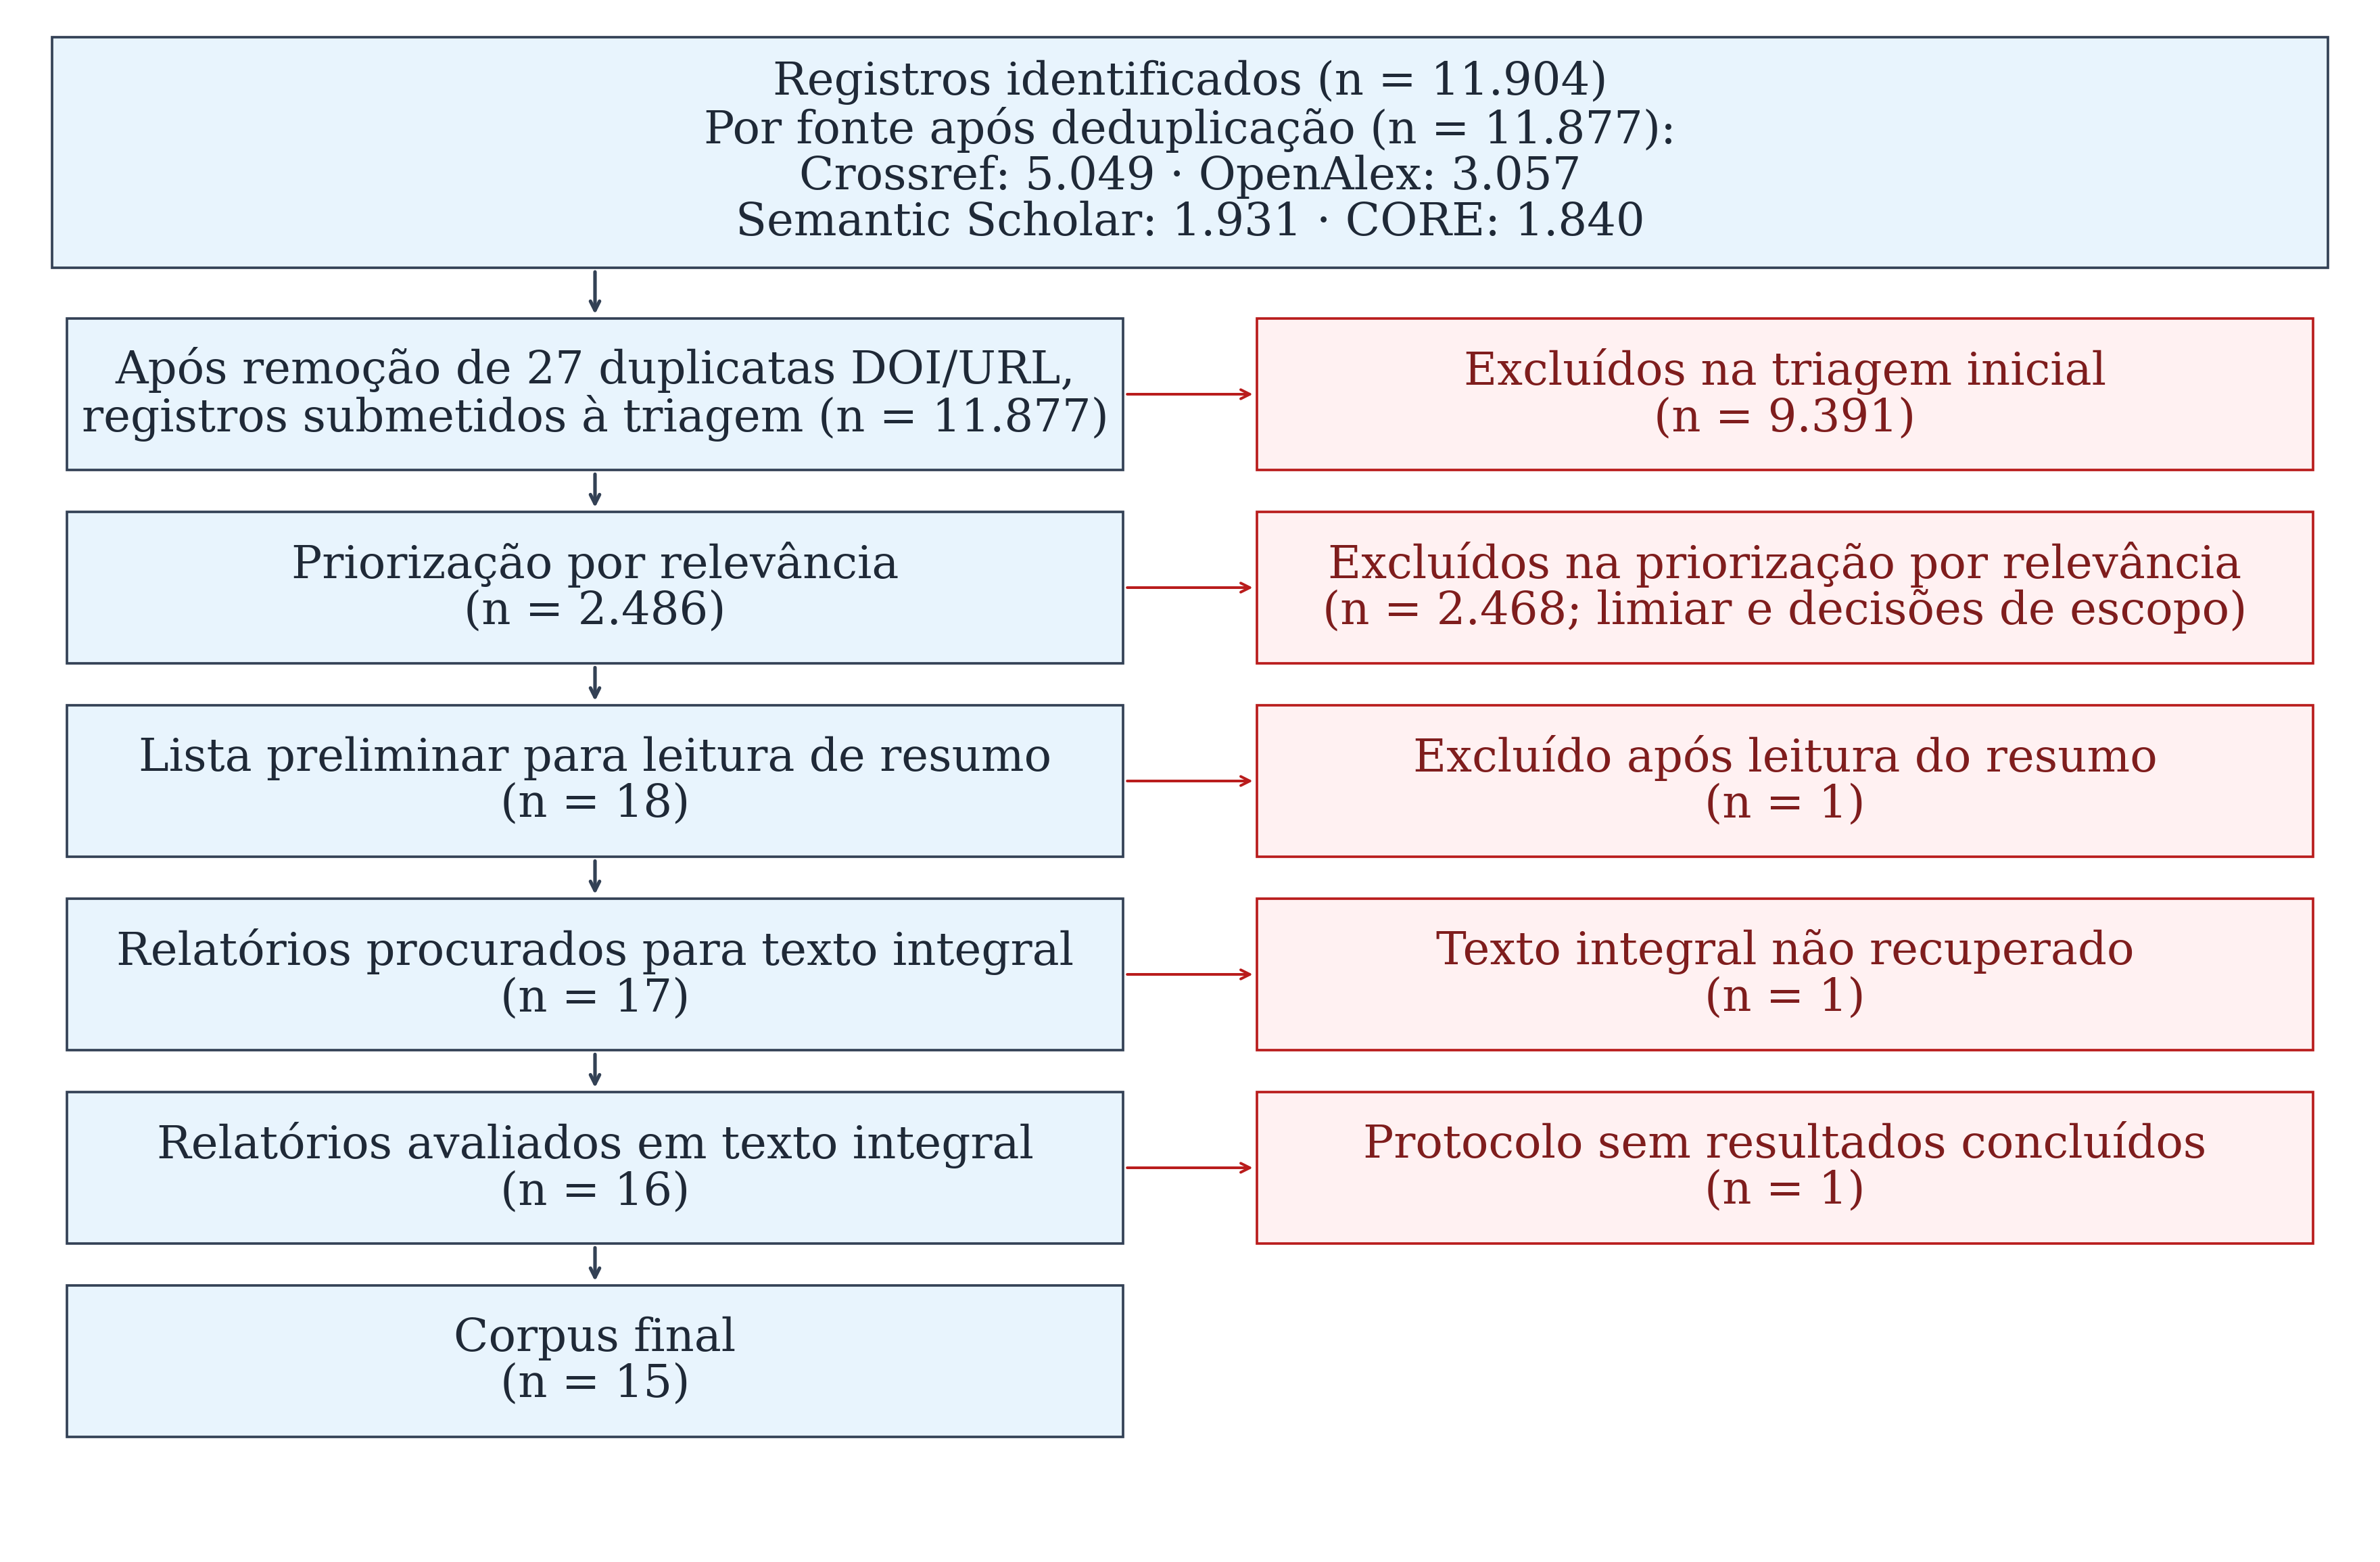
\includegraphics[width=\textwidth]{images/prisma_flow.png}
\fonte{Elaborado pelo autor (2026).}
\end{fluxograma}

\section{Estatísticas Descritivas}

A Tabela~\ref{tab:stats-descritivas} reúne os principais números da revisão. A auditoria de identidade registra as remoções determinísticas que entram no fluxo PRISMA e mantém separadas as repetições observadas apenas por título. Depois da remoção por DOI/URL, permaneceram 232 excedentes em grupos de título normalizado, tratados como candidatos à revisão semântica e não como duplicatas confirmadas. A pequena proporção de registros retidos decorreu do escopo específico e da aplicação do filtro operacional de relevância temática, seguida da verificação de escopo.

A taxa de acertos do \textit{cache} não foi apresentada como métrica fixa. Um acerto ocorreu quando uma consulta foi atendida com uma resposta previamente armazenada, sem nova requisição à API. Como essa proporção dependeu do histórico de execução, sua interpretação permaneceu vinculada aos contadores registrados em cada execução do sistema.

\begin{table}[H]
\centering
\caption{Estatísticas descritivas da revisão sistemática.}
\label{tab:stats-descritivas}
\begin{tabular}{lc}
\hline
\textbf{Métrica} & \textbf{Valor} \\
\hline
Registros identificados & 11.904 \\
Remoções determinísticas por DOI/URL & 27 (0,23\%) \\
Registros na triagem & 11.877 \\
Excluídos na triagem & 9.391 (78,89\%) \\
Registros submetidos à priorização operacional & 2.486 \\
Excluídos na priorização operacional & 2.468 (99,28\%) \\
Registros retidos operacionalmente & 18 \\
Candidatos empíricos provisórios & 17 \\
Protocolo/proposta contextual & 1 \\
Bases consultadas & 4 \\
Consultas bilíngues & 72 (48 EN + 24 PT) \\
Período de cobertura & 2015--2026 \\
\hline
\end{tabular}
\fonte{Elaborado pelo autor (2026).}
\end{table}

Os percentuais da tabela usam denominadores explicitados para evitar a leitura de taxas de etapas diferentes como se fossem equivalentes: 27 remoções correspondem a 0,23\% dos 11.904 registros identificados; 9.391 exclusões na triagem correspondem a 78,89\% dos mesmos 11.904 registros identificados; e 2.468 exclusões correspondem a 99,28\% dos 2.486 registros submetidos à priorização operacional. Assim, o percentual da triagem descreve a parcela dos registros inicialmente identificados, não a proporção excluída apenas entre os registros efetivamente triados.

A distribuição por fonte é apresentada no Gráfico~\ref{fig:database-coverage}. O universo representado corresponde aos 11.877 registros do snapshot após a remoção determinística por DOI/URL, e não aos 11.904 registros brutos identificados. A fonte indica a procedência registrada para a representação preservada no snapshot; não mede a cobertura exclusiva de cada base nem a qualidade dos estudos. As quantidades e proporções foram calculadas a partir do export versionado, sem nova coleta.

\begin{grafico}[H]
\centering
\caption{Registros do snapshot após deduplicação, por fonte científica.}
\label{fig:database-coverage}
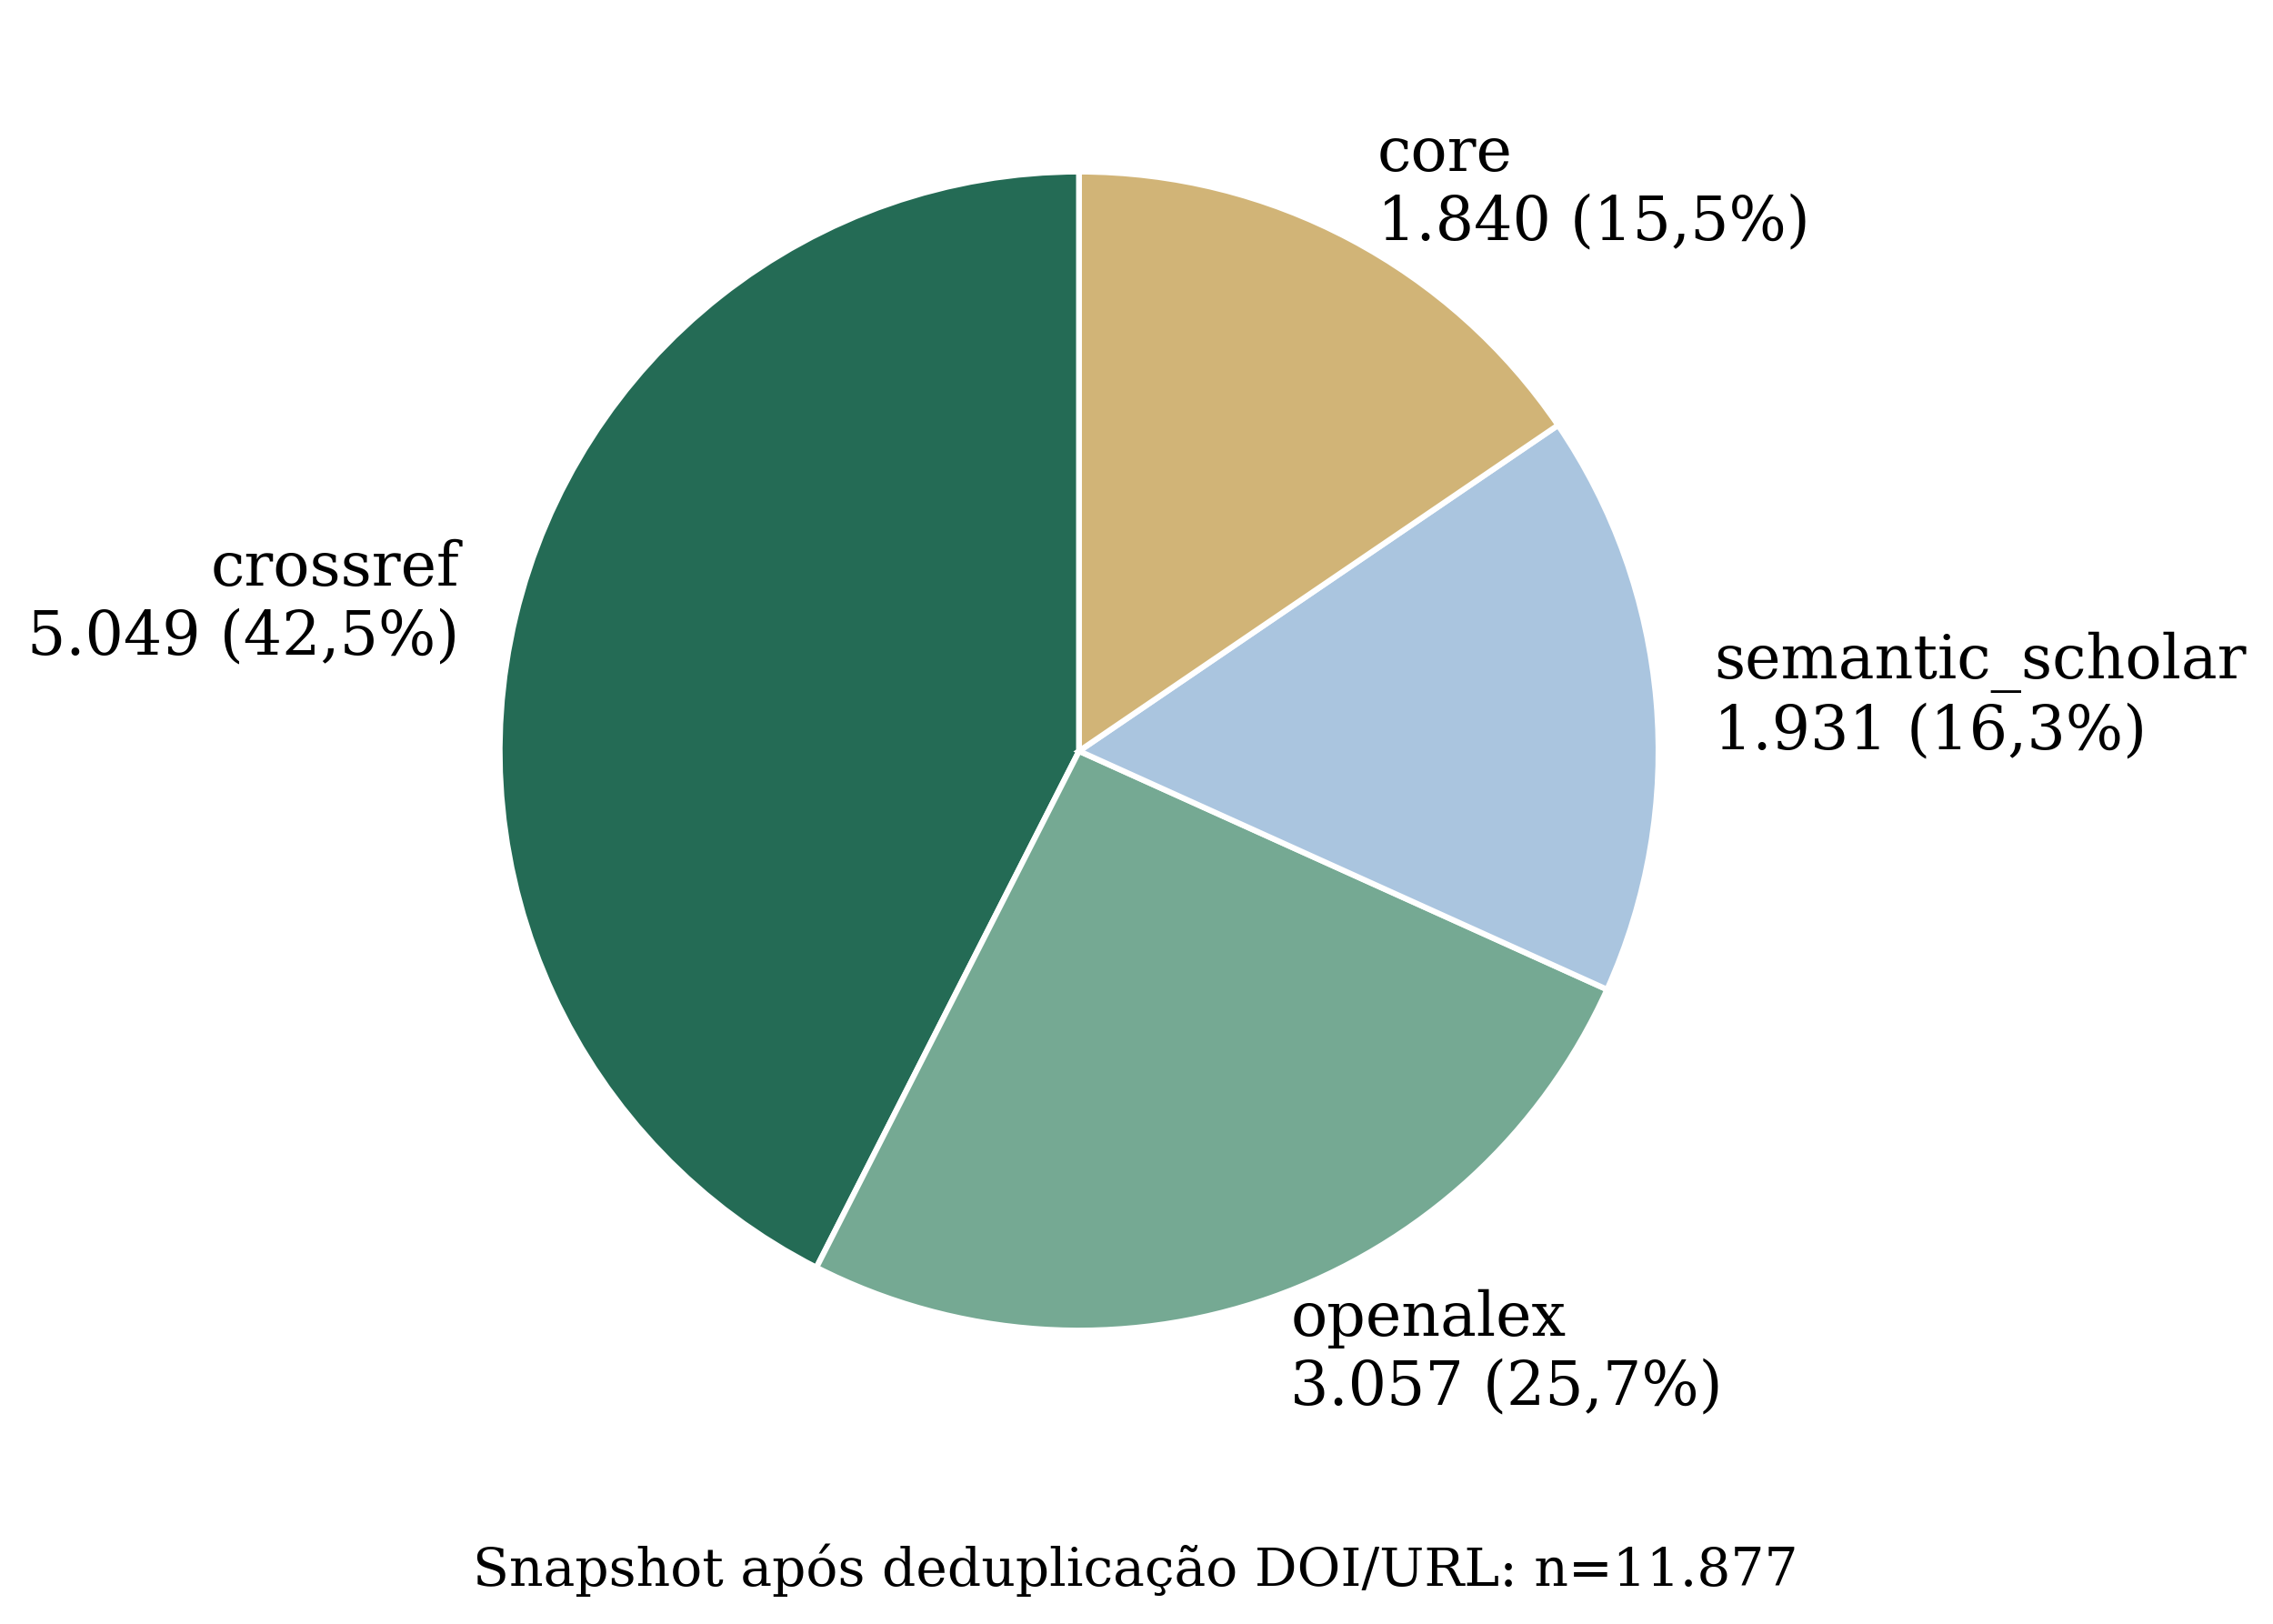
\includegraphics[width=0.85\textwidth]{images/database_coverage.png}
\fonte{Elaborado pelo autor (2026).}
\end{grafico}

\section{Síntese dos Candidatos Empíricos Provisórios}

Entre os candidatos analisados, foram identificadas tarefas de predição de desempenho e de classificação ou estimativa de proficiência. Os estudos empregaram métodos diversos, incluindo \textit{Random Forest}, SVM, árvores de decisão e redes neurais. Seus resultados não são diretamente comparáveis em todos os casos, pois foram produzidos com populações, instrumentos, variáveis e desenhos metodológicos distintos.

Os trabalhos preditivos utilizaram combinações de notas, respostas a itens, características contextuais e registros de interação para estimar categorias ou escores. Outros estudos investigaram personalização, avaliação formativa, recursos pedagógicos ou modelos computacionais de aprendizagem. Essa diversidade ampliou o panorama da revisão, mas também impediu tratar todos os resultados como se medissem o mesmo fenômeno educacional.

Acurácia elevada em uma base específica não demonstra automaticamente que a técnica produzirá o mesmo resultado em outra escola ou população. Da mesma forma, predição de desempenho não equivale a explicar como o estudante aprende matemática. Essas restrições foram incorporadas aos requisitos e aos critérios de avaliação da especificação apresentada no Capítulo~\ref{cap:prototipo}.

No Quadro~\ref{qua:sintese-estudos-empiricos}, a coluna “Síntese do relato consultado” resume a informação localizada para cada estudo. Conforme o conteúdo recuperado, essa síntese pode descrever objetivo, abordagem, resultado ou limite documental; não constitui uma medida harmonizada de efeito nem permite comparar a eficácia entre estudos. A leitura deve considerar conjuntamente o desenho, a finalidade, a população analisada e as limitações metodológicas apresentadas na apreciação MMAT. O protocolo contextual de \citeonline{Imperatrice2025_6921} foi mantido para rastreabilidade, mas não integra o quadro por não apresentar resultado empírico concluído.

O estudo de \citeonline[pp.~8--9, 13--14, 18, 24]{UniversityMathematics2026_6919} é evidência empírica adjacente: descreve uma reforma de matemática universitária aplicada à metrologia de carbeto de silício e um questionário adaptativo que os autores denominam baseado em IA. A comparação usa uma coorte de controle de 2021 (n=94) e uma coorte pós-reforma de 2025 (n=89), separadas por quatro anos. Embora os autores relatem indicadores de linha de base sem diferenças estatisticamente significativas, o desenho não contemporâneo não elimina confundimento temporal, e o artigo reconhece possíveis mudanças de equipe e contexto. Assim, os resultados não isolam o efeito do questionário ou da IA, nem demonstram eficácia generalizável de tutoria personalizada. O texto consultado não especifica um algoritmo de aprendizado de máquina; por isso, o estudo não é classificado como evidência de ML.

\begingroup
\fontsize{10}{11.5}\selectfont
\setlength{\tabcolsep}{2pt}
\renewcommand{\arraystretch}{1.05}
\def\LTcaptype{quadro}
\setlength{\LTcapwidth}{\textwidth}
\setlength{\LTleft}{0pt}
\setlength{\LTright}{\fill}
\begin{longtable}{>{\raggedright\arraybackslash}p{\dimexpr0.17\textwidth-2\tabcolsep\relax}>{\raggedright\arraybackslash}p{\dimexpr0.22\textwidth-2\tabcolsep\relax}>{\raggedright\arraybackslash}p{\dimexpr0.17\textwidth-2\tabcolsep\relax}>{\raggedright\arraybackslash}p{\dimexpr0.14\textwidth-2\tabcolsep\relax}>{\raggedright\arraybackslash}p{\dimexpr0.30\textwidth-2\tabcolsep\relax}}
\caption{Síntese dos candidatos empíricos provisórios retidos.}\label{qua:sintese-estudos-empiricos}\\
\hline
\textbf{Autores/Ano} & \textbf{Tema e finalidade} & \textbf{Abordagem} & \textbf{Avaliação} & \textbf{Síntese do relato consultado} \\
\hline
\endfirsthead
\multicolumn{5}{c}{\quadroname\ \thequadro\ -- Continuação}\\
\hline
\textbf{Autores/Ano} & \textbf{Tema e finalidade} & \textbf{Abordagem} & \textbf{Avaliação} & \textbf{Síntese do relato consultado} \\
\hline
\endhead
\hline
\multicolumn{5}{r}{\textit{Continua na próxima página}}\\
\endfoot
\hline
\endlastfoot
\citeonline{Implementation2025_000} & Predição de desempenho acadêmico em matemática.\newline Finalidade: Predição & EDM; ML; classificadores & Acurácia & 75\% no conjunto de teste reportado \\
\citeonline{Math2021_001} & Proficiência matemática no PISA 2012 computadorizado.\newline Finalidade: Predição de proficiência & ML multiclasse; RN; RF & Kappa; ROC-AUC & Comparação entre modelos de três classes, conforme resumo do autor \\
\citeonline{He2025_6915} & Tecnologia educacional para matemática.\newline Finalidade: Otimização e decisão & EDM; IA; modelos preditivos & Meta-análise; modelagem; comparação escolar & Predição de tamanhos de efeito e aplicação em oito turmas \\
\citeonline{Villegas2025_6916} & Tutoria inteligente em STEM.\newline Finalidade: Feedback personalizado & IA; aprendizagem adaptativa & Desempenho; análise estatística & Sistema adaptativo avaliado no contexto descrito pelo estudo \\
\citeonline{Multimodels2020_002} & Desempenho em matemática no ensino médio.\newline Finalidade: Predição & EDM; ML; métodos estatísticos & Comparação de modelos & Estudo compara classes de métodos em dados escolares \\
\citeonline{Analysis2022_003} & Desempenho em conjuntos escolares de Matemática e Língua Portuguesa.\newline Finalidade: Predição & DT; JRip; NB; MLP; RF & Acurácia; comparação & Seleção de atributos e comparação de classificadores em dois domínios \\
\citeonline{Ozseven2026_6917} & Desempenho em matemática on-line.\newline Finalidade: Predição & ML; modelo neurofuzzy & Desempenho preditivo & Estrutura híbrida para lidar com incerteza e generalização \\
\citeonline{Design2025_004} & Trajetórias personalizadas em cursos de Matemática, Chinês e Inglês.\newline Finalidade: Personalização & DL; grafo de conhecimento; RL; análise de sentimento & Desempenho reportado no resumo indexado & O resumo reporta comparação com grupo de controle; texto integral e método não foram recuperados para conferência \\
\citeonline{Innovative2023_005} & Currículo de matemática superior apoiado por IA.\newline Finalidade: Personalização & ACO; CNN; CRF; grafo de conhecimento & Análise estatística; feedback & Modelo de trajetória personalizada descrito e avaliado no estudo \\
\citeonline{Identifying2017_006} & Classificação de desempenho no TIMSS 2011.\newline Finalidade: Classificação & RF; J48; Naive Bayes; MLP; regressão logística & Classificação & A lista de modelos difere entre a tabela e a configuração experimental do artigo \\
\citeonline{Machine2019_007} & Analítica preditiva em STEM.\newline Finalidade: Predição de desempenho & Oito algoritmos de ML & Benchmarking & Benchmark reportado no resumo; texto integral não recuperado, contexto matemático não confirmado \\
\citeonline{Computational2017_008} & Modelagem computacional da aprendizagem em frações e equações.\newline Finalidade: Simulação e predição qualitativa & Modelos comparados com registros de tutoria & Ajuste de modelos; AIC; BIC & Efeitos instrucionais previstos qualitativamente, sem escores absolutos de desempenho \\
\citeonline{Machine2024_009} & Apoio ao ensino de matemática.\newline Finalidade: Classificação de estudantes & ML; árvore de decisão & Predição de desempenho & Heurística de classificação do sucesso matemático \\
\citeonline{UniversityMathematics2026_6919} & Matemática universitária e desenvolvimento sustentável.\newline Finalidade: Integração curricular & Questionário adaptativo descrito como IA; Fourier; PCA & Desempenho, questionário e entrevistas & Reforma curricular com aplicação industrial; coortes históricas sem isolamento do efeito computacional \\
\citeonline{Echeveria2025_6920} & Mentalidade matemática e intervenção precoce.\newline Finalidade: Classificação de mentalidade & EDM; NB; SVM; MLP & Acurácia & Modelo de classificação com questionários e dados acadêmicos \\
\citeonline{Enhancing2025_012} & Teoremas de círculo.\newline Finalidade: Ensino de geometria & Animação computacional; aprendizagem cooperativa & Quase-experimento & Comparação entre animação com jigsaw e ensino convencional \\
\citeonline{Zeng2025_6923} & Carga cognitiva na resolução de problemas matemáticos.\newline Finalidade: Reconhecimento de estados cognitivos & EEG; rastreamento ocular; ML & Experimento intraindivíduos & Sinais multimodais e classificadores para reconhecer carga cognitiva \\
\end{longtable}
\fonte{Elaborado pelo autor (2026).}
\endgroup

Os resultados quantitativos requerem leitura junto aos seus denominadores e às métricas por classe. Em \citeonline[pp.~155--156, 160]{Implementation2025_000}, o alvo é a categoria da nota escolar de matemática, em uma amostra de 280 estudantes de uma escola privada. Os autores descrevem uma divisão de 70\% para treinamento e 30\% para teste e reportam 75\% de acurácia de teste para a combinação de SMOTE e RUSBoost. Na mesma comparação, a revocação da classe de baixo desempenho é de 43\%. Portanto, a acurácia agregada não caracteriza uniformemente a identificação das três classes, nem demonstra ganho de aprendizagem decorrente de uma intervenção.

Em \citeonline[pp.~1, 16, 31--35]{He2025_6915}, convém distinguir três componentes do artigo: a síntese meta-analítica de 423 publicações, a predição de tamanhos de efeito e a aplicação escolar em oito turmas. As publicações examinadas pelos autores não foram adicionadas como registros da presente revisão, e o alvo da modelagem foi o tamanho de efeito de uma intervenção, não a proficiência individual. As inconsistências de denominador e de unidade analítica da aplicação escolar são examinadas na Seção~\ref{sec:tendencias-lacunas}.

A tese de \citeonline[pp.~44--48, 56]{Computational2017_008} contribui como referência conceitual e metodológica para a modelagem computacional da aprendizagem. Nas tarefas de frações, compara simulações com registros de tutoria previamente coletados no DataShop para 79 estudantes e prevê qualitativamente efeitos de sequenciamentos instrucionais, não escores absolutos de desempenho no tutor ou em pós-teste. Em análise distinta sobre resolução de equações, descreve dados de 71 estudantes e 10.052 passos; a análise utiliza 4.568 passos nos quais os estudantes executaram as próprias ações, enquanto tarefas de estratégia em que o tutor realizava as transformações ficam fora desse recorte. Portanto, sua contribuição está delimitada às tarefas examinadas e não constitui avaliação prospectiva nem evidência de eficácia do protótipo deste TCC.

\section{Avaliação Metodológica com o MMAT}
\label{sec:qualidade-estudos}

O MMAT 2018 foi aplicado conforme o delineamento de cada estudo empírico, com consulta ao artigo de apresentação e ao guia oficial \cite{MMAT2018,MMATGuide2018}. O ledger registra as perguntas de triagem S1 e S2 e os critérios específicos Q1--Q5, sem média, ranking ou categoria geral. As respostas são Y (``Sim''), N (``Não''), CT (``Não é possível concluir com a evidência disponível'') ou, exclusivamente para o protocolo contextual 6921, N/A (``Não aplicável''). A apreciação é de revisor único e permanece preliminar: cinco candidatos foram examinados com base em resumos e metadados, os localizadores por critério ainda requerem consolidação e a adjudicação independente está pendente. Os estudos 6916, 6919 e 6920 foram identificados como métodos mistos; além dos critérios da categoria mista, o quadro complementar apresenta apreciações separadas dos componentes qualitativo e quantitativo. Esses julgamentos também aguardam revisão independente e não constituem classificação definitiva dos artigos.

Os Quadros~\ref{qua:mmat-reavaliacao-atual} e~\ref{qua:mmat-componentes} são gerados dos arquivos versionados \path{research/data/mmat_reassessment_current.csv} e \path{research/data/mmat_component_reassessment_current.csv}. Eles mantêm os critérios da categoria mista separados das apreciações dos componentes e da avaliação histórica.

\begingroup
\fontsize{10}{11.5}\selectfont
\setlength{\tabcolsep}{3pt}
\renewcommand{\arraystretch}{1.0}
% Reserva a abertura antes de longtable criar a âncora da legenda.
% Sem espaço, o destino pode ficar na página anterior no TeX Live.
\Needspace{18\baselineskip}
% Quadro gerado de research/data/mmat_reassessment_current.csv
% Reavaliação documental preliminar; não representa score nem avaliação final.
% Não editar manualmente; execute: python -m src.analysis.mmat_current_tcc_table
\begingroup
\SingleSpacing
\setlength{\parindent}{0pt}
\fontsize{10}{12}\selectfont
\def\LTcaptype{quadro}
\setlength{\tabcolsep}{2pt}
\setlength{\LTcapwidth}{\textwidth}
\begin{longtable}{|>{\raggedright\arraybackslash}p{4.5cm}|>{\raggedright\arraybackslash}p{4.5cm}|ccccccc|}
\caption{Triagem e apreciação preliminar pelo MMAT 2018 de 15 estudos do corpus.}\label{qua:mmat-reavaliacao-atual}\\
\hline
\textbf{Estudo} & \textbf{Desenho} & \textbf{S1} & \textbf{S2} & \textbf{Q1} & \textbf{Q2} & \textbf{Q3} & \textbf{Q4} & \textbf{Q5} \\
\hline
\endfirsthead
\multicolumn{9}{c}{\quadroname\ \thequadro\ -- Continuação}\\
\hline
\textbf{Estudo} & \textbf{Desenho} & \textbf{S1} & \textbf{S2} & \textbf{Q1} & \textbf{Q2} & \textbf{Q3} & \textbf{Q4} & \textbf{Q5} \\
\hline
\endhead
\hline
\multicolumn{9}{r}{\textit{Continua na próxima página}}\\
\endfoot
\hline
\endlastfoot
\citeonline{Math2021_001} & Quant. descritivo & Y & Y & Y & CT & CT & CT & CT \\
\citeonline{Implementation2025_000} & Quant. descritivo & Y & Y & Y & CT & CT & CT & Y \\
\citeonline{Multimodels2020_002} & Quant. descritivo & Y & Y & CT & CT & CT & CT & CT \\
\citeonline{Analysis2022_003} & Quant. descritivo & Y & Y & CT & CT & CT & CT & CT \\
\citeonline{Design2025_004} & Cat. 3 utilizada (alocação incerta) & Y & Y & CT & CT & CT & CT & CT \\
\citeonline{Identifying2017_006} & Quant. descritivo & Y & Y & Y & CT & CT & CT & CT \\
\citeonline{Innovative2023_005} & Cat. 3 utilizada (alocação incerta) & Y & Y & CT & CT & CT & CT & CT \\
\citeonline{Computational2017_008} & Cat. 4 adaptada (modelagem) & Y & Y & Y & CT & CT & CT & CT \\
\citeonline{Machine2024_009} & Quant. descritivo & Y & Y & CT & CT & CT & CT & CT \\
\citeonline{Enhancing2025_012} & Cat. 2 declarada (contraditória) & Y & Y & CT & N & Y & CT & CT \\
\citeonline{He2025_6915} & Quant. não rand. (componente escolar) & Y & Y & CT & Y & CT & N & Y \\
\citeonline{Villegas2025_6916} & Métodos mistos & Y & Y & Y & Y & CT & CT & CT \\
\citeonline{Ozseven2026_6917} & Quant. descritivo & Y & Y & Y & CT & CT & CT & Y \\
\citeonline{UniversityMathematics2026_6919} & Métodos mistos & Y & Y & Y & Y & N & CT & N \\
\citeonline{Echeveria2025_6920} & Métodos mistos & Y & Y & Y & Y & CT & CT & N \\
\end{longtable}
\fonte{Elaborado pelo autor (2026).}
\par\noindent\textit{Nota:} S1/S2 = perguntas de triagem; Q1--Q5 = critérios da categoria; Y = sim; N = não; CT = não é possível concluir; Quant. = quantitativo; rand. = randomizado. Ver Seção~\ref{sec:avaliacao-qualidade}.\par
\endgroup

% Quadro gerado de research/data/mmat_component_reassessment_current.csv
\begingroup
\SingleSpacing
\setlength{\parindent}{0pt}
\def\LTcaptype{quadro}
\fontsize{10}{12}\selectfont
\setlength{\tabcolsep}{2pt}
\renewcommand{\arraystretch}{1.15}
\begin{longtable}{|>{\raggedright\arraybackslash}p{2.2cm}|>{\raggedright\arraybackslash}p{2.2cm}|ccccc|>{\raggedright\arraybackslash}p{6.1cm}|}
\caption{Componentes qualitativos e quantitativos dos estudos de métodos mistos.}\label{qua:mmat-componentes}\\
\hline
\textbf{Estudo} & \textbf{Componente} & \textbf{C1} & \textbf{C2} & \textbf{C3} & \textbf{C4} & \textbf{C5} & \textbf{Síntese e páginas consultadas} \\
\hline
\endfirsthead
\multicolumn{8}{c}{\quadroname\ \thequadro\ -- Continuação}\\
\hline
\textbf{Estudo} & \textbf{Componente} & \textbf{C1} & \textbf{C2} & \textbf{C3} & \textbf{C4} & \textbf{C5} & \textbf{Síntese e páginas consultadas} \\
\hline
\endhead
\hline
\multicolumn{8}{r}{\textit{Continua na próxima página}}\\
\endfoot
\hline
\endlastfoot
\citeonline{Villegas2025_6916} & Quant. não rand. & CT & CT & CT & CT & CT & 3.1 (CT): A população de recrutamento e a estratégia de amostragem não estão estabelecidas nas seções examinadas. 3.2 (CT): As medidas de resultado são descritas, mas o relato disponível não fundamenta suficientemente sua adequação. 3.3 (CT): A completude dos dados de resultado e as perdas de participantes não estão estabelecidas. 3.4 (CT): A alocação dos grupos e o controle inicial de fatores de confusão não estão suficientemente documentados. 3.5 (CT): A introdução menciona um semestre acadêmico, os métodos relatam seis semanas e os resultados mostram progresso na oitava semana para estudantes de programação com alta interação; essa divergência não estabelece a adesão ou a cronologia do componente de matemática. Páginas e seções: Páginas físicas 2 (450 estudantes e semestre letivo), 13–16 (delineamento, medidas e análise), 18–23 (resultados; semana 8 na p. 22) e 24–27 (testes e limites) \\
\citeonline{Villegas2025_6916} & Qualitativo & Y & Y & CT & CT & CT & 1.1 (Y): A abordagem qualitativa é pertinente para examinar as percepções de estudantes e educadores sobre o sistema de tutoria. 1.2 (Y): Entrevistas estruturadas com estudantes e educadores, realizadas ao fim da experiência e com tópicos pertinentes explicitados, são adequadas para explorar as percepções sobre o sistema (página física 16). Detalhes de seleção e registro continuam como perguntas de esclarecimento, sem serem tratados automaticamente como inadequação da coleta. 1.3 (CT): O relato menciona análise temática e temas, mas não explicita suficientemente a derivação analítica a partir das entrevistas (páginas físicas 16–17). 1.4 (CT): As interpretações das entrevistas não são suficientemente vinculadas ao material qualitativo examinado (páginas físicas 16–17); médias e percentuais de satisfação nas pp. 24–25 são dados quantitativos e não resolvem esse vínculo. 1.5 (CT): A coerência entre fontes qualitativas, coleta, análise e interpretação permanece pouco clara. Páginas e seções: Páginas físicas 16–17 (Qualitative Analysis); 24–25 (satisfação quantitativa, não dados de entrevista) \\
\citeonline{UniversityMathematics2026_6919} & Quant. não rand. & CT & Y & CT & N & CT & 3.1 (CT): Os grupos pertencem a uma disciplina e estão separados por quatro anos. O artigo menciona amostragem por conglomerados, mas não define a população-alvo nem explica como as turmas de 2021 e 2025 foram escolhidas (páginas físicas 7–8). 3.2 (Y): O questionário e os resultados da disciplina são descritos e analisados; a apreciação permanece provisória. 3.3 (CT): A completude e o tratamento dos dados de resultado não estão suficientemente documentados nas seções examinadas. 3.4 (N): Os grupos de controle e experimental de anos diferentes introduzem confundimento temporal reconhecido pelos autores; os testes de linha de base não controlam mudanças de equipe, contexto e uso de IA (páginas físicas 8 e 24). 3.5 (CT): A implementação da intervenção e a adesão não estão suficientemente documentadas para este critério. Páginas e seções: Páginas físicas 7–8 (§4.1.1), 12–14 (§4.3–4.4.1, tabela 4) e 24 (§6) \\
\citeonline{UniversityMathematics2026_6919} & Qualitativo & Y & Y & CT & Y & CT & 1.1 (Y): As entrevistas são adequadas para explorar as perspectivas dos estudantes sobre a reforma da disciplina. 1.2 (Y): O artigo relata entrevistas semiestruturadas com 12 estudantes do grupo experimental, selecionados aleatoriamente logo após o curso (página física 18). 1.3 (CT): As etapas analíticas utilizadas para derivar os temas não estão suficientemente detalhadas. 1.4 (Y): A interpretação inclui relatos dos estudantes e é apoiada por citações apresentadas no artigo (página física 18). 1.5 (CT): A relação entre amostragem qualitativa, coleta, análise e conclusões integradas requer verificação adicional. Páginas e seções: Páginas físicas 18 (§4.4.8) e 24 (§6) \\
\citeonline{Echeveria2025_6920} & Quant. descritivo & Y & CT & N & CT & CT & 4.1 (Y): Os registros de estudantes de uma escola são adequados à questão de classificação local descrita no estudo. 4.2 (CT): A escola e seus estudantes delimitam uma população local; o MMAT não exige uma população-alvo mais abrangente. A correspondência dos 428 casos completos aos 633 recrutados não foi estabelecida, com anos letivos divergentes e sem comparação suficiente dos retidos e não retidos (páginas físicas 3 e 7). 4.3 (N): Oito itens da escala usados para construir as categorias de mentalidade também permanecem entre os preditores selecionados, comprometendo a mensuração independente do alvo. 4.4 (CT): O relato informa 633 participantes recrutados e 428 casos completos e cita os anos letivos 2023–2024 e 2022–2023 sem esclarecer a origem dos grupos nem se os casos ausentes produzem viés de não resposta. 4.5 (CT): As descrições da divisão dos dados e da validação divergem e não permitem apreciar claramente a adequação da análise. Páginas e seções: Páginas físicas 3/\allowbreak{}impressa 65 (§2.1–2.3), 6/\allowbreak{}68 (§2.6) e 7–8/\allowbreak{}69–70 (resultados) \\
\citeonline{Echeveria2025_6920} & Qualitativo & Y & Y & CT & Y & CT & 1.1 (Y): As entrevistas com professores são pertinentes aos objetivos declarados de contextualização e triangulação do estudo. 1.2 (Y): O relato identifica entrevistas com cinco docentes de Matemática para explorar o uso do modelo e apresenta suas falas individuais (páginas físicas 3 e 11–12), constituindo coleta pertinente à questão de percepção docente. A seleção e o registro das respostas permanecem pouco detalhados. 1.3 (CT): O procedimento analítico do material das entrevistas não está adequadamente descrito. 1.4 (Y): As falas individuais dos docentes sustentam a interpretação descritiva de suas percepções sobre identificação, apoio e planejamento (páginas físicas 11–12). O julgamento não transforma expectativas dos entrevistados em efeito observado sobre aprendizagem. 1.5 (CT): A coerência entre fontes, coleta, análise e interpretação qualitativas não pode ser concluída, pois o procedimento de análise das entrevistas permanece pouco explicitado (páginas físicas 3 e 11–13). A integração com dados quantitativos é examinada separadamente nos critérios de métodos mistos. Páginas e seções: Páginas físicas 3/\allowbreak{}impressa 65 (§2.1 e coleta), 11–12/\allowbreak{}73–74 (falas docentes) e 13/\allowbreak{}75 (conclusões) \\
\end{longtable}
\fonte{Elaborado pelo autor (2026).}
\par\noindent\textit{Nota:} C1--C5 = critérios da categoria; Y = sim; N = não; CT = não é possível concluir; Quant. = quantitativo; rand. = randomizado. Ver Seção~\ref{sec:avaliacao-qualidade}.\par
\endgroup

\fonte{Elaborado pelo autor (2026).}
\endgroup

Os julgamentos preliminares por critério registraram limitações relativas à descrição dos dados, ao controle de variáveis de confusão e à representatividade. Como a avaliação foi conduzida por um único revisor e a disponibilidade de textos primários foi desigual, esses registros não foram convertidos em uma estimativa de frequência nem em classificação agregada de qualidade.

A recuperação adicional de fontes não implica aprovação dos julgamentos anteriores. Para \citeonline[pp.~1, 16, 31--35]{He2025_6915}, o ledger delimita provisoriamente a apreciação ao componente escolar da aplicação, classificado como quantitativo não randomizado; os demais componentes do artigo não integram essa unidade de avaliação. Na categoria quantitativa não randomizada, o MMAT 2018 inclui critérios sobre controle de confundidores e administração da intervenção conforme planejada \cite{MMAT2018}. A classificação do delineamento e as respostas por critério permanecem preliminares e aguardam adjudicação independente; portanto, não representam uma apreciação definitiva do artigo como um todo.

\section{Tendências e Lacunas}
\label{sec:tendencias-lacunas}

As observações desta seção consideram somente os 17 candidatos empíricos provisórios; o protocolo ou proposta contextual foi mantido para rastreabilidade e não integra a síntese de evidências. A leitura é descritiva e foi limitada pela disponibilidade desigual das fontes: doze registros tiveram o texto primário consultado e cinco foram apreciados com base em resumo e metadados. Os exemplos a seguir localizam limitações em estudos específicos; essa cobertura não permite estimar a frequência das limitações na literatura, comparar a eficácia das intervenções ou afirmar que o conjunto apresenta evidência homogênea.

Em \citeonline[pp.~1, 16, 31--35]{He2025_6915}, a descrição da aplicação escolar informa oito turmas com 45 estudantes cada, o que corresponde a 360 estudantes por cálculo aritmético, enquanto o artigo declara amostra total de 90. O texto consultado não reconcilia esses denominadores. Os autores também descrevem quatro professores, com um deles responsável pelas duas turmas de controle e os demais pelas turmas experimentais; não foi identificado ajuste para esse possível confundimento entre docente e condição nas páginas examinadas. Além disso, embora o artigo reporte testes \textit{t} independentes para grupos de 45 estudantes, organiza as condições por turma e não informa se a análise considera esse agrupamento. Não é possível, portanto, reconstruir a unidade analítica nem a precisão das comparações. Esses limites do relato exigem cautela, sem autorizar corrigir o denominador por inferência ou declarar os resultados inválidos.

Em \citeonline[pp.~1, 14, 22]{Villegas2025_6916}, a introdução descreve a avaliação em um semestre acadêmico, a seção de métodos informa período experimental de seis semanas e os resultados apresentam, na subanálise de programação, progresso até a oitava semana para estudantes com alta interação. O relato não reconcilia essas janelas temporais; portanto, o resultado de programação não deve ser transportado para matemática nem usado para fixar uma duração única do estudo. Já \citeonline[pp.~101--105]{Enhancing2025_012} apresenta descrições incompatíveis sobre a alocação das escolas: um trecho informa distribuição aleatória, e outro caracteriza o desenho como quase-experimental sem alocação aleatória. O artigo também relata diferença entre os grupos no pré-teste (U=6714; p<0,001; tamanho de efeito=0,346), e a intervenção combina animação computacional e aprendizagem cooperativa. Em conjunto, esses elementos limitam a atribuição do resultado a um componente isolado e recomendam que a comparação seja interpretada considerando a diferença inicial e a intervenção combinada.

Em \citeonline[pp.~65, 69--70]{Echeveria2025_6920}, a seção de métodos situa a matrícula no ano letivo de 2023--2024, enquanto a seção~3.1 associa os 633 estudantes ao ano letivo de 2022--2023, sem esclarecer se são coortes distintas. Esse conflito não deve ser conciliado por inferência. Além disso, oito itens da escala de mentalidade matemática utilizados para formar as categorias também permanecem entre os preditores selecionados. O relato não estabelece, por si só, validade diagnóstica independente da classificação; por isso, o resultado não sustenta inferência de mudança na aprendizagem nem de efeito de uma intervenção precoce.

Esses casos sugerem requisitos de relato e avaliação para a especificação: explicitar denominadores, unidades de análise, alocação, medidas iniciais, duração e relação entre rótulos e preditores. Eles são exemplos localizados, não uma estimativa de prevalência nem uma avaliação definitiva dos estudos. Temas mais amplos — como equidade, participação docente, integração curricular e reprodutibilidade — não foram codificados de modo comparável para todos os registros; neste trabalho, permanecem questões e requisitos propostos para investigação, e não ausências demonstradas em toda a literatura ou em cada estudo retido.

\section{Limitações e Contribuições da Revisão}

A revisão foi realizada por um único pesquisador, com suporte automatizado para deduplicação, triagem e organização dos registros. Não houve dupla revisão independente. A priorização operacional de grande parte dos registros foi avaliada a partir de títulos, resumos e metadados, pois nem todos os textos completos estavam disponíveis; por isso, a retenção não deve ser apresentada como elegibilidade final universal.

O protocolo não foi registrado prospectivamente. Foram adotados princípios de planejamento compatíveis com o PRISMA-P, mas não se afirmou conformidade integral. O PRISMA 2020 foi utilizado para orientar o relato do processo.

As fontes consultadas possuem cobertura predominantemente anglófona, e a busca foi limitada a português e inglês. A heterogeneidade dos desenhos, populações e métricas impediu uma síntese quantitativa conjunta. Não foi aplicado um teste formal de viés de publicação; a cobertura das fontes e a disponibilidade desigual dos textos completos podem ter influenciado o conjunto recuperado. Além disso, a apreciação MMAT por revisor único permanece preliminar e está sujeita a divergências interpretativas.

Considerados esses limites, a revisão forneceu a base documental disponível para a especificação do protótipo. A presença de tarefas preditivas entre os candidatos analisados justificou considerar modelos supervisionados como alternativas, enquanto a heterogeneidade das bases fundamentou critérios de seleção e validação. Requisitos de explicabilidade, integração curricular, participação docente e reprodutibilidade foram propostos a partir da leitura temática e da fundamentação pedagógica; como esses aspectos não foram codificados de modo comparável em todos os registros, não são apresentados como lacunas comprovadas em cada estudo ou em toda a literatura.

Dessa forma, os resultados da revisão não foram tratados apenas como levantamento bibliográfico. Eles sustentaram as decisões consolidadas no Capítulo~\ref{cap:prototipo}, preservando a distinção entre evidências reportadas na literatura e resultados produzidos pelo próprio trabalho.

%--------- FIM REVISÃO SISTEMÁTICA ------------

\chapter{ESPECIFICAÇÃO DO PROTÓTIPO}
\label{cap:prototipo}

Este capítulo apresenta a especificação conceitual do protótipo elaborada a partir dos resultados da revisão sistemática e da fundamentação pedagógica. O artefato produzido consolidou princípios de projeto, requisitos funcionais e não funcionais, critérios para fontes de dados e modelos, um protocolo de avaliação e uma arquitetura de referência.

O repositório também contém uma implementação técnica do fluxo automatizado do protótipo, acompanhada por testes sintéticos automatizados. Essa implementação verifica comportamentos de processamento e de proteção contra falhas nos casos sintéticos testados, mas não equivale a uma execução com dados educacionais reais, a uma validação de eficácia preditiva ou a uma avaliação de aprendizagem. O capítulo, portanto, descreve a especificação que orienta uma futura execução e mantém essa implementação técnica separada de qualquer alegação de resultado educacional.

\section{Princípios e Requisitos}
\label{sec:principios-requisitos}

A especificação estabelece que o protótipo deverá apoiar a decisão pedagógica sem substituir o professor. Essa decisão de projeto implica distinguir, na representação e na interpretação dos resultados, o desempenho observado em uma atividade, a proficiência estimada por um modelo, a competência mobilizada em um contexto mais amplo e a aprendizagem como possível mudança ao longo do tempo.

As estimativas deverão ser acompanhadas de explicações, limitações e condições de validade compreensíveis para seus destinatários. A revisão humana deverá permanecer integrada ao uso das recomendações, de modo que o professor possa confrontar as evidências com o contexto da turma e decidir se há fundamento para uma intervenção.

A proteção dos dados educacionais constitui outro princípio da especificação. O uso deverá estar associado a uma finalidade explícita, com minimização dos dados pessoais e controle de acesso compatível com essa finalidade. Também deverá ser possível reproduzir e auditar os procedimentos de preparação, treinamento e avaliação por meio do registro das versões, dos parâmetros e das dependências relevantes. A especificação também rejeita rótulos permanentes que convertam uma estimativa situada em característica fixa do estudante.

No plano funcional, a futura implementação deverá importar dados documentados e relacionados a objetivos curriculares, preservando os metadados necessários à leitura de sua procedência. A partir desses dados, deverá organizar evidências de desempenho por habilidade ou descritor, de modo que a análise mantenha relação explícita com o contexto curricular em que os registros foram produzidos.

Na etapa de análise, o protótipo deverá produzir estimativas para um alvo educacional explicitamente definido, acompanhadas de incertezas e limitações, e apresentar resultados individuais e agregados ao professor. Uma probabilidade preditiva de acerto ou de pertencimento a uma classe de desempenho não será denominada proficiência apenas por resultar de um modelo computacional. A interpretação como proficiência exigirá um modelo de mensuração, uma escala e evidências de validade para o uso pretendido, em consonância com a distinção entre observação e inferência discutida por \citeonline[p.~42--44]{NRC2001}. Essas saídas deverão explicar as variáveis relacionadas a cada estimativa. Por fim, deverá exportar dados, parâmetros e resultados para auditoria das versões, decisões e saídas.

No plano não funcional, a especificação estabelece condições de qualidade e de governança para a implementação futura. A reprodutibilidade deverá ser assegurada pelo registro das versões dos dados, dos parâmetros, dos modelos e das dependências. Complementarmente, a rastreabilidade deverá permitir associar cada resultado à fonte de dados utilizada e à versão do experimento que o produziu. Essa associação é necessária para que uma conclusão possa ser examinada sem perder sua procedência.

A testabilidade deverá ser favorecida pela separação entre ingestão, preparação, modelagem, avaliação e apresentação. A portabilidade, por sua vez, exigirá um ambiente de execução documentado e passível de reprodução. Essas condições permitem verificar e repetir os procedimentos em diferentes formas de implementação.

Os requisitos também abrangem a relação do protótipo com seus usuários e com os dados tratados. A apresentação deverá ser acessível, compreensível e compatível com diferentes perfis de usuário. A privacidade deverá orientar a minimização de dados pessoais e o controle de finalidade e de acesso. Por fim, a transparência deverá exigir que as limitações dos modelos e as condições de validade das estimativas sejam comunicadas junto aos resultados, evitando que a forma de apresentação atribua uma certeza que o procedimento não sustenta.

A escolha de fontes de dados permanece condicionada à documentação disponível, ao problema de pesquisa e às condições de execução que vierem a ser definidas. A especificação considera a possibilidade de trabalhar com microdados de avaliações educacionais, como SAEB e PISA, e com dados sintéticos destinados à verificação do fluxo automatizado; a seleção definitiva depende dessas condições.

A implementação técnica exploratória do repositório segue uma escolha distinta, de viabilidade, que não substitui esse critério. Seu adaptador aceita somente a versão corrigida do conjunto \textit{Skill-builder data 2009-2010} do ASSISTments\footnote{Página do conjunto, cuja URL o provedor pede que seja citada: \url{https://sites.google.com/site/assistmentsdata/home/2009-2010-assistment-data/skill-builder-data-2009-2010}. Acesso em: 22 out. 2026.}, que registra uma linha por par estudante--problema, com ordem das interações, indicador de acerto e habilidades associadas. O sistema que gerou esses registros é descrito por \citeonline{Feng2009}, referência indicada pelo próprio provedor, embora esse artigo não analise o conjunto de 2009--2010. A escolha atende a uma verificação técnica do fluxo de previsão da próxima resposta, que exige registros sequenciais por habilidade; os microdados de proficiência do SAEB e do PISA não têm essa estrutura. Ela não seleciona a base de uma investigação empírica, não representa estudantes brasileiros e não foi acompanhada do processamento de qualquer arquivo real nesta versão; as demais fontes aparecem na configuração apenas como candidatas, sem adaptador implementado. Os termos de uso publicados pelo provedor deverão ser registrados e respeitados antes de qualquer aquisição.

A seleção de uma fonte deverá considerar, inicialmente, sua licença e suas condições de uso, bem como a existência de dicionário de dados e de documentação metodológica. Também deverá examinar a unidade de análise e sua relação com o problema de pesquisa, a qualidade dos metadados e o tratamento previsto para valores ausentes. A representatividade da população deverá ser analisada em relação ao contexto para o qual se pretende interpretar os resultados, sem ser presumida a partir da simples disponibilidade da base. Do mesmo modo, a presença de variáveis relacionadas ao desempenho e ao contexto educacional será relevante, mas não garantirá, por si só, que seja possível associá-las a competências ou descritores curriculares. Essa associação deverá ser demonstrada e delimitada pela documentação e pelo desenho da avaliação.

Por fim, a análise da fonte deverá incluir os riscos de identificação, discriminação e uso indevido. Esses riscos são condições de governança da execução, e não apenas atributos técnicos do arquivo de dados. Dados sintéticos poderão ser usados para testar fluxos de processamento, interfaces e regras de validação.

Quanto à modelagem, a revisão identificou uso de \textit{Random Forest}, máquinas de vetores de suporte (SVM), árvores de decisão, regressão logística e redes neurais. Na especificação, \textit{Random Forest} e SVM também foram ancoradas em suas fontes metodológicas primárias \cite{Breiman2001,CortesVapnik1995}. Modelos supervisionados simples e interpretáveis foram mantidos como referências iniciais de comparação, condicionando o uso de modelos mais complexos à demonstração de ganho e à possibilidade de interpretação adequada.

\textit{Random Forest} e SVM foram registrados como alternativas de modelagem, não como algoritmos definitivamente implementados. A escolha entre eles depende da base selecionada, da distribuição das classes, do tipo de variável, do custo computacional e dos requisitos de explicabilidade.

O código exploratório não implementa essas duas alternativas. Ele contém referências históricas simples, uma regressão logística regularizada \cite{James2021} e, como candidato não linear exploratório, um classificador que combina modelos ajustados sequencialmente (\textit{gradient boosting}) \cite{Friedman2001} em sua variante baseada em histogramas disponível na biblioteca scikit-learn \cite{Pedregosa2011}. Essa composição foi definida para testar o fluxo com um modelo interpretável e um candidato não linear; não resulta de uma comparação com \textit{Random Forest} ou SVM nem indica superioridade de qualquer modelo. Nenhum desses modelos foi treinado com dados educacionais reais.

\section{Protocolo de Avaliação da Especificação Conceitual}
\label{sec:protocolo-avaliacao}

O protocolo proposto para o OE4 examina a especificação conceitual; sua aplicação permanece pendente. O procedimento deverá examinar a rastreabilidade dos requisitos até as fontes ou decisões autorais, a consistência entre entradas, saídas e responsabilidades da arquitetura e a correspondência entre as saídas previstas e os conceitos educacionais adotados. A viabilidade será examinada documentalmente pelas condições necessárias de acesso e uso dos dados, disponibilidade de variáveis, recursos computacionais e participação docente.

Para cada requisito examinado, deverão ser registrados seu identificador, a versão da especificação, a fonte e a localização no texto (página ou seção), o critério utilizado, a justificativa e a necessidade de ajuste. O julgamento poderá indicar coerência documental, coerência condicionada a ressalvas ou necessidade de revisão; falta de evidência deverá permanecer explícita, sem ser convertida em aprovação. A revisão por docentes e a análise técnica deverão ser registradas separadamente, com discussão das divergências. O Quadro~\ref{qua:rastreabilidade-requisitos} organiza os requisitos a serem examinados nesse procedimento.

\label{sec:avaliacao-empirica-futura}

Para uma futura execução e avaliação do protótipo com dados educacionais reais, um protocolo experimental distinto deverá orientar a modelagem e a interpretação dos seus resultados. Ele deverá separar o que será observado no comportamento técnico dos modelos daquilo que exigiria evidência educacional adicional. Essa separação começa pela definição explícita dos conjuntos de treino, validação e teste e pela prevenção de vazamento de informação entre preparação, modelagem e avaliação. Os modelos candidatos deverão ser comparados com referências simples, para que diferenças de desempenho, inclusive resultados nulos ou desfavoráveis, sejam interpretadas em relação a uma base de comparação, e as métricas deverão ser analisadas por classe, além das medidas agregadas, quando a tarefa permitir essa decomposição.

Como descrição complementar dos erros e acertos, o protocolo prevê o uso de matriz de confusão, precisão, revocação e medida F1. A área sob a curva ROC e a calibração somente deverão ser calculadas quando forem compatíveis com a tarefa e com o tipo de saída produzido \cite{Fawcett2006,NiculescuMizilCaruana2005}. Também deverão ser examinadas a estabilidade das explicações e possíveis diferenças entre grupos, sem converter essas análises em conclusões causais não sustentadas pelo desenho do estudo. Por fim, a execução deverá registrar as limitações de generalização relacionadas à fonte de dados, à população observada e às condições de aplicação.

Para examinar a adequação pedagógica da especificação, o protocolo prevê uma revisão documental por docentes da área de matemática. Essa revisão deverá considerar a correspondência dos requisitos com o referencial curricular pertinente ao nível de ensino, a clareza das explicações e das incertezas apresentadas, a possibilidade de interpretação contextualizada e a preservação da decisão docente. Cada julgamento deverá registrar o requisito examinado, a evidência documental, a justificativa, as limitações e os ajustes necessários.

Como parte da avaliação e da revisão humana, SHAP e LIME foram incluídos como alternativas para explicar modelos, com referência às formulações originais de Lundberg e Lee e de Ribeiro, Singh e Guestrin \cite{LundbergLee2017,RibeiroSinghGuestrin2016}. Seu uso deverá considerar a estabilidade das explicações, o custo computacional e a possibilidade de tradução dos resultados para uma linguagem curricular compreensível. A implementação exploratória não inclui SHAP nem LIME, que permanecem alternativas especificadas. Para a regressão logística, ela decompõe o logaritmo da razão de chances de cada previsão em intercepto e produtos entre coeficientes e valores transformados dos atributos. Essa decomposição é exata para esse modelo linear. Também calcula a importância por permutação no conjunto de teste, adaptando o procedimento proposto por \citeonline{Breiman2001} para florestas aleatórias a outros tipos de modelo. O candidato de \textit{gradient boosting} não possui explicação implementada.

O procedimento de revisão docente não foi executado neste trabalho e não substituiria um estudo empírico de eficácia educacional. As condições para interpretar as saídas técnicas estão reunidas na Seção~\ref{sec:limitacoes-revisao}.

\section{Arquitetura de Referência}
\label{sec:arquitetura-prototipo}

A ingestão corresponde à leitura das fontes, à validação inicial de seus formatos e à preservação das informações de procedência. Em seguida, a etapa de preparação deverá tratar valores ausentes, codificar e transformar variáveis e documentar as decisões tomadas sobre esses dados. A modelagem abrangerá o treinamento e a comparação dos modelos candidatos de acordo com a base selecionada e com o protocolo de avaliação.

A etapa de avaliação e explicabilidade deverá calcular as métricas, analisar os erros e gerar explicações cuja estabilidade e limitações serão examinadas. Por fim, a apresentação deverá disponibilizar indicadores, incertezas e limitações de modo compreensível para a análise docente. Essa arquitetura organiza responsabilidades e pontos de verificação para a implementação futura, sem fixar tecnologia ou forma de implantação.

A separação dos componentes deverá favorecer a testabilidade, a rastreabilidade e a substituição controlada de técnicas. Ela também permite localizar em qual etapa uma decisão, uma transformação ou uma limitação foi introduzida. A arquitetura não impõe uma interface específica e poderá ser materializada como caderno computacional interativo, aplicação local, API ou sistema web. Essas formas de execução deverão preservar os requisitos da Seção~\ref{sec:principios-requisitos}.

\section{Fundamentação e Rastreabilidade dos Requisitos}
\label{sec:rastreabilidade-requisitos}

A especificação articula três origens que não devem ser confundidas: observações localizadas nos estudos do corpus, fundamentos teóricos ou normativos e decisões de projeto do autor. Um problema de relato identificado em um artigo pode motivar uma salvaguarda, mas não demonstra que a solução proposta seja eficaz. Da mesma forma, um referencial pedagógico orienta a interpretação das saídas sem validar uma interface ou um algoritmo específico.

O Quadro~\ref{qua:rastreabilidade-requisitos} organiza os requisitos das seções anteriores em 26 grupos identificáveis. A coluna de origem explicita a base da decisão e a última coluna delimita a inferência permitida. Requisitos de engenharia que não receberam sustentação externa específica são apresentados como escolhas autorais, e não como achados empíricos da revisão. As referências remetem aos trabalhos discutidos na fundamentação e na síntese; as páginas ou seções que sustentam as apreciações empíricas estão indicadas no registro de evidências dos estudos.

Os grupos R01--R19 remetem aos requisitos e critérios da Seção~\ref{sec:principios-requisitos}; R07, R10, R11 e R16 também explicitam condições da arquitetura na Seção~\ref{sec:arquitetura-prototipo}. R20--R26 correspondem às condições do protocolo de avaliação da Seção~\ref{sec:protocolo-avaliacao}. Esses vínculos identificam onde cada grupo foi especificado, sem transformar as decisões autorais em exigências extraídas de um artigo.

\begingroup
\def\LTcaptype{quadro}
\fontsize{8.5}{10.5}\selectfont
\setlength{\tabcolsep}{3pt}
\renewcommand{\arraystretch}{1.15}
\setlength{\LTcapwidth}{\textwidth}
\begin{longtable}{|>{\raggedright\arraybackslash}p{0.7cm}|>{\raggedright\arraybackslash}p{3.0cm}|>{\raggedright\arraybackslash}p{4.4cm}|>{\raggedright\arraybackslash}p{5.7cm}|}
\caption{Origem, derivação e limites dos requisitos da especificação conceitual.}\label{qua:rastreabilidade-requisitos}\\
\hline
\textbf{Cód.} & \textbf{Requisito ou grupo} & \textbf{Origem e base documental} & \textbf{Derivação e limite da justificativa} \\
\hline
\endfirsthead
\multicolumn{4}{c}{\quadroname\ \thequadro\ -- Continuação}\\
\hline
\textbf{Cód.} & \textbf{Requisito ou grupo} & \textbf{Origem e base documental} & \textbf{Derivação e limite da justificativa} \\
\hline
\endhead
\hline
\multicolumn{4}{r}{\textit{Continua na próxima página}}\\
\endfoot
\hline
\endlastfoot
R01 & Apoio docente e revisão humana, sem prescrição autônoma. & Fundamento teórico e decisão autoral: mediação em \citeonline{Vygotsky1978} e \citeonline{WoodBrunerRoss1976}. & A mediação orienta a participação do professor; não demonstra utilidade do protótipo nem mensuração da zona de desenvolvimento proximal. \\
\hline
R02 & Separar desempenho, previsão, proficiência, competência e aprendizagem. & Fundamento teórico e normativo: \citeonline[p.~42--44]{NRC2001}, \citeonline{OECDPISA2022Framework} e \citeonline{BNCC2018}. & Exigir construto e validade para interpretar inferências. A definição operacional de aprendizagem adotada neste trabalho não foi testada pelo protótipo. \\
\hline
R03 & Comunicar explicações, incertezas e condições de validade. & Fundamento teórico e decisão autoral: \citeonline{NRC2001} e \citeonline{HattieTimperley2007}. & Informação interpretável é condição proposta de uso. Explicação algorítmica não equivale automaticamente a retorno pedagógico formativo compreendido pelo docente. \\
\hline
R04 & Finalidade, minimização, acesso e análise de riscos de identificação e uso indevido. & Fundamento normativo e decisão de governança: \citeonline{LGPD2018}. & Orientar o planejamento do tratamento de dados pessoais; não declarar conformidade jurídica de uma implementação ainda não avaliada. \\
\hline
R05 & Evitar rótulos permanentes e interpretações discriminatórias. & Fundamento teórico e salvaguarda autoral: limites de inferência em \citeonline{NRC2001}. & Restringir a interpretação à tarefa e ao contexto; não afirmar dano demonstrado no corpus nem equidade já alcançada. \\
\hline
R06 & Registrar versões, parâmetros e dependências; exportar dados e resultados, vinculando cada saída à fonte e à versão do experimento. & Decisão de projeto do autor, explicitada nos princípios e requisitos deste capítulo. & Viabilizar inspeção documental e reprodução futura. O corpus não demonstra a eficácia desse conjunto operacional. \\
\hline
R07 & Importar dados documentados e preservar procedência. & Decisão de projeto do autor, relativa à ingestão e à preparação. & Preservar contexto e registrar validações de formato; não presumir qualidade pelo simples sucesso da importação. \\
\hline
R08 & Relacionar evidências a habilidades, descritores e objetivos curriculares. & Fundamento teórico e normativo: \citeonline{BNCC2018} e \citeonline{Ausubel1968}; aplicação operacional autoral. & Orientar o vínculo curricular e considerar conhecimentos anteriores. A associação concreta entre variáveis e habilidades ainda deverá ser demonstrada. \\
\hline
R09 & Definir o alvo e distinguir saídas individuais de agregadas. & Observação do corpus: alvos e unidades distintos em \citeonline[p.~11--12, seção de definição do resultado predito]{He2025_6915}; fundamento em \citeonline{NRC2001}; decisão autoral de apresentação. & A predição de efeito de intervenções não equivale à proficiência individual. A forma de exibição ainda não foi avaliada com docentes. \\
\hline
R10 & Separar componentes para favorecer testabilidade. & Decisão de arquitetura do autor: ingestão, preparação, modelagem, avaliação e apresentação. & Organizar responsabilidades e pontos de inspeção; não tratar modularidade como propriedade empiricamente comprovada da proposta. \\
\hline
R11 & Documentar o ambiente e permitir substituição controlada de técnicas. & Decisão de projeto do autor sobre portabilidade e interfaces. & Condicionar execução à documentação de dependências e contratos; a especificação não demonstra portabilidade entre ambientes reais. \\
\hline
R12 & Considerar acessibilidade e diferentes perfis de usuários. & Requisito autoral de apresentação, sem validação específica no corpus. & Registrar uma condição a operacionalizar em critérios de aceitação; não declarar acessibilidade alcançada ou avaliada. \\
\hline
R13 & Examinar SAEB e PISA como fontes candidatas, não definitivas. & Exemplo do corpus em \citeonline{Math2021_001}; documentação contextual de \citeonline{SAEB2021} e \citeonline{PISA2022}; decisão autoral. & Uso de uma edição do PISA não valida outra base, outra edição ou sua transferência ao contexto brasileiro. O uso do ASSISTments no código exploratório é teste de viabilidade, não seleção da base. \\
\hline
R14 & Verificar licença, condições de uso, dicionário e documentação metodológica. & Critério autoral para seleção das fontes. & Condicionar uso à documentação e às permissões pertinentes. Disponibilidade pública e proteção de dados não substituem licença de uso. \\
\hline
R15 & Examinar unidade de análise e representatividade da população. & Observação do corpus: seleção e alvo em \citeonline[p.~50]{Math2021_001}; distinção de unidades em \citeonline[p.~11--12, seção de definição do resultado predito]{He2025_6915}; decisão autoral. & Exigir compatibilidade entre pergunta, amostra e inferência. Casos localizados não estimam a frequência de problemas na literatura. \\
\hline
R16 & Documentar metadados, transformações e valores ausentes. & Decisão de projeto do autor para seleção e preparação de dados. & Tornar as decisões examináveis; não fixar regra universal de imputação nem garantir validade das variáveis. \\
\hline
R17 & Restringir dados sintéticos à verificação técnica. & Delimitação autoral do escopo e do protocolo proposto. & Verificar fluxos e regras sem inferir aprendizagem, validade preditiva em dados reais ou eficácia pedagógica. \\
\hline
R18 & Considerar famílias supervisionadas como alternativas. & Exemplos do corpus em \citeonline[p.~1609, algoritmos de classificação]{Identifying2017_006} e \citeonline[p.~156, Tabela~2]{Implementation2025_000}; fontes metodológicas \cite{Breiman2001,CortesVapnik1995}. & Identificar candidatos, condicionando a escolha ao tipo de variável, à distribuição das classes, ao custo e à explicabilidade. A ocorrência em artigos não estabelece superioridade ou adequação. \\
\hline
R19 & Comparar com referências simples e justificar complexidade. & Fundamento metodológico em \citeonline{James2021}; regra de comparação autoral. & Interpretar ganhos sob condições explícitas; não antecipar algoritmo vencedor ou limiar universal de ganho aceitável. \\
\hline
R20 & Separar treino, validação e teste e prevenir vazamento. & Fundamento metodológico em \citeonline{James2021}; relato contraditório de \citeonline[p.~50--51]{Math2021_001}. & A ambiguidade documental motiva separação e relato inequívocos; não permite determinar qual procedimento foi efetivamente executado no artigo. \\
\hline
R21 & Examinar confusão, precisão, revocação e F1 por classe. & Resultados por classe em \citeonline[p.~160, Tabela~8]{Implementation2025_000}; fundamento em \citeonline{James2021}; decisão autoral de protocolo. & Examinar erros que a acurácia agregada pode ocultar; resultados de uma base não determinam o desempenho futuro do protótipo. \\
\hline
R22 & Usar ROC-AUC e calibração quando compatíveis com a tarefa. & Fundamentos metodológicos em \citeonline{Fawcett2006} e \citeonline{NiculescuMizilCaruana2005}. & Distinguir discriminação e qualidade probabilística; nenhuma das métricas constitui medida de aprendizagem. \\
\hline
R23 & Examinar estabilidade das explicações e diferenças entre grupos. & Decisão autoral de avaliação, orientada pelos limites de validade discutidos em \citeonline{NRC2001}. & Formular verificações futuras, cujo procedimento ainda deverá ser operacionalizado. Desempenho médio não demonstra estabilidade ou equidade. \\
\hline
R24 & Delimitar generalização e evitar causalidade automática. & Observações localizadas em \citeonline[p.~50]{Math2021_001}, \citeonline[p.~5, seção~2.2]{Machine2024_009} e \citeonline[p.~654, conclusão]{Design2025_004}; interpretação crítica autoral. & Restringir a conclusão à população, ao alvo e ao desenho examinados; não transformar associação ou ganho relatado em efeito causal. \\
\hline
R25 & Prever revisão documental por docentes e registrar julgamentos. & Referencial curricular em \citeonline{BNCC2018} e avaliação formativa em \citeonline{HattieTimperley2007}; procedimento proposto pelo autor. & Examinar adequação curricular e interpretativa da especificação. O procedimento não foi executado e não substituiria avaliação de eficácia educacional. \\
\hline
R26 & Examinar SHAP e LIME, sua estabilidade, custo e comunicação curricular. & Fontes metodológicas \cite{LundbergLee2017,RibeiroSinghGuestrin2016}; escolha autoral de alternativas. & Identificar métodos de explicação, sem atribuir às fontes prova de compreensão docente, estabilidade ou adequação curricular da aplicação proposta. O código exploratório implementa apenas a decomposição exata da regressão logística e a importância por permutação. \\
\hline
\end{longtable}
\endgroup
\fonte{Elaborado pelo autor (2026).}

O quadro torna verificável a origem declarada de cada grupo, mas não encerra a apreciação científica das referências. Permanecem distintas a rastreabilidade documental, a conferência da interpretação de cada fonte e a avaliação futura do artefato. Os critérios funcionais, os cenários e a regra de revisão docente estão definidos nas Seções~\ref{sec:aceitacao-funcional} e~\ref{sec:revisao-docente-operacional}. A aplicação e as verificações de acessibilidade e estabilidade explicativa permanecem etapas futuras.


%--------- FIM ESPECIFICAÇÃO DO PROTÓTIPO ------------

\chapter{RESULTADOS E DISCUSSÃO}
\label{cap:resultados-discussao}

Este capítulo integra a revisão sistemática, a apreciação metodológica, os fundamentos pedagógicos e a especificação do protótipo. A discussão relaciona essas entregas ao problema de pesquisa e aos objetivos.

\section{Síntese dos Resultados}

A revisão caracterizou tarefas de predição e avaliação de resultados matemáticos, como a classificação com itens do PISA por \citeonline{Math2021_001} e a previsão de resultados em uma disciplina por \citeonline{Machine2024_009}. Também reuniu propostas de personalização, como a de \citeonline{Design2025_004}, e a experiência universitária de \citeonline{UniversityMathematics2026_6919}, que articula Transformada de Fourier à medição de carbeto de silício (SiC). O Fluxograma~\ref{fig:prisma-flow} apresenta a seleção do corpus.

A apreciação metodológica manteve respostas S1/S2 e cinco critérios específicos para os 15 estudos empíricos, sem pontuação geral, média ou ranking. Essa apresentação permite examinar descrição dos dados, representatividade, completude, controle de confundidores e integração de métodos por estudo. As categorias adaptadas e as restrições das fontes estão explicitadas na Seção~\ref{sec:limitacoes-revisao}.

A fundamentação distinguiu desempenho observado, proficiência estimada, competência e aprendizagem. Notas, acertos, tentativas e tempos de resposta são evidências associadas à tarefa e ao contexto; a interpretação de conhecimentos e habilidades depende do construto e do instrumento \cite{NRC2001}. A probabilidade preditiva de um alvo definido foi distinguida do desempenho observado. Conhecimento prévio, mediação, avaliação formativa e retorno pedagógico orientaram requisitos de explicabilidade, revisão humana, associação curricular, proteção de dados e comunicação de incertezas.

A especificação reuniu princípios, requisitos funcionais e não funcionais, critérios de seleção de dados, alternativas de modelagem, protocolo de avaliação e arquitetura de referência. Os componentes abrangem ingestão, preparação, modelagem, avaliação, explicabilidade e apresentação. O Quadro~\ref{qua:rastreabilidade-requisitos} relaciona observações dos estudos, fundamentos teóricos ou normativos e decisões de projeto. Dados sintéticos foram reservados à verificação técnica do fluxo.

\section{Atendimento aos Objetivos}

No escopo executado, o primeiro objetivo específico foi desenvolvido por meio da categorização das técnicas e finalidades pedagógicas no Capítulo~\ref{cap:revisao}. O segundo foi desenvolvido pela identificação de limitações no material examinado. O terceiro foi operacionalizado nos requisitos, critérios para dados e modelos e arquitetura do Capítulo~\ref{cap:prototipo}. O quarto resultou na proposição do protocolo de avaliação da viabilidade e da coerência da especificação, apresentado na Seção~\ref{sec:protocolo-avaliacao}. Sua aplicação não foi realizada; o protocolo experimental de uma eventual implementação constitui uma possibilidade separada.

O componente propositivo do objetivo geral foi realizado no escopo documental pela elaboração de uma especificação técnica e pedagógica para apoiar a interpretação docente da aprendizagem matemática. Sua fundamentação permanece preliminar, em razão da seleção automatizada por relevância, do histórico incompleto das consultas, do relatório não recuperado e da apreciação MMAT ainda sujeita à conferência. Assim, a entrega é uma especificação derivada tematicamente do conjunto analisado, sem representar síntese conclusiva da literatura ou solução educacional validada.

\section{Discussão Integrada}

A leitura da literatura orientou a escolha de não selecionar uma técnica apenas por sua frequência de uso ou pela maior acurácia reportada. Na especificação, a seleção considera qualidade e representatividade dos dados, finalidade pedagógica, possibilidade de interpretação e condições de aplicação.

As tarefas de classificação e estimativa foram relacionadas aos conceitos educacionais da fundamentação. O professor participa da interpretação das saídas, considerando fatores pedagógicos, sociais e contextuais que o modelo não observa diretamente. Essa organização permite discutir contribuições computacionais sem atribuir aos autores dos estudos uma posição teórica uniforme.

A contribuição integra revisão sistemática, apreciação metodológica, fundamentação pedagógica e engenharia de requisitos. A seleção de algoritmos permanece subordinada ao contexto de uso e à avaliação; os limites das evidências estão reunidos na Seção~\ref{sec:limitacoes-revisao}.

%--------- FIM RESULTADOS E DISCUSSÃO ------------

\chapter{CONCLUSÃO}
\label{cap:conclusao}

Este trabalho investigou técnicas computacionais aplicadas ao ensino de matemática e elaborou uma especificação conceitual de protótipo. A revisão caracterizou aplicações de classificação e predição, como as de \citeonline{Math2021_001} e \citeonline{Machine2024_009}, propostas de trajetórias personalizadas, como a de \citeonline{Design2025_004}, e integração computacional ao ensino universitário, como a de \citeonline{UniversityMathematics2026_6919}. O Fluxograma~\ref{fig:prisma-flow} sintetiza a formação do corpus.

A entrega propositiva tomou a forma de uma especificação técnica e pedagógica voltada à interpretação docente da aprendizagem matemática. Ela articula a categorização das técnicas, os limites encontrados na literatura, os requisitos e a arquitetura de referência. Também propõe um protocolo para examinar a viabilidade e a coerência da especificação. Esse conjunto atende ao componente propositivo do objetivo geral no escopo documental do trabalho.

Entre as contribuições, destacam-se a síntese estruturada, os dados e o código versionados e a apreciação MMAT por critérios, separada da relevância temática. A fundamentação distinguiu desempenho observado, probabilidade preditiva, proficiência estimada, competência e aprendizagem. Essa distinção orientou critérios de explicabilidade, participação docente, avaliação e proteção de dados na especificação.

As limitações delimitam o alcance dessas contribuições. A fundamentação da especificação permanece preliminar: o fluxo automatizado não permite reconstruir integralmente as consultas históricas, o relatório de \citeonline{Zeng2025_6923} não foi recuperado e as 15 triagens e os 15 conjuntos de critérios MMAT ainda precisam de conferência humana. As categorias utilizadas para \citeonline{Design2025_004}, \citeonline{Innovative2023_005}, \citeonline{Computational2017_008} e \citeonline{Enhancing2025_012} mantêm as restrições descritas na Seção~\ref{sec:limitacoes-revisao}. A tese de MacLellan foi considerada como um relatório com componentes matemáticos, sem duplicar frações reutilizadas. A revisão e a especificação não constituem uma síntese conclusiva da literatura nem uma solução educacional validada. Não houve aplicação funcional com base definitiva ou participantes, e os testes sintéticos da implementação exploratória não demonstram eficácia pedagógica.

Como continuidade, propõe-se concluir a conferência das fontes e dos julgamentos MMAT e aplicar o protocolo de avaliação da especificação. Uma eventual aplicação educacional dependerá de decisão posterior, seleção de dados compatíveis e comparação de modelos de referência em ambiente reproduzível. Estudos com participantes exigirão avaliação ética aplicável, autorização institucional, proteção dos dados e participação de profissionais da educação.

A continuidade poderá examinar estabilidade das explicações, diferenças de desempenho entre grupos, alinhamento curricular e utilidade das informações para o planejamento docente. Essas atividades ampliam a revisão e a especificação entregues, preservando o professor como responsável pela interpretação pedagógica e pelas decisões de intervenção.

%--------- FIM CONCLUSÃO ------------


% ----------------------------------------------------------
% ELEMENTOS PÓS-TEXTUAIS
% ----------------------------------------------------------
\postextual

\bibliography{referencias,referencias_pedagogicas}
\begin{apendicesenv}

\chapter{MAPEAMENTO DO RELATO AO PRISMA 2020}
\label{apendice:prisma-checklist}

Este apêndice apresenta um mapeamento do relato deste manuscrito com base no PRISMA 2020 \cite{PRISMA2020}. O quadro desdobra os 27 itens do checklist em suas alíneas aplicáveis e utiliza tópicos abreviados; os requisitos completos estão no \href{https://www.prisma-statement.org/prisma-2020-checklist}{checklist oficial}. O mapeamento avalia o que foi apresentado no texto, não certifica a execução do procedimento, o rigor metodológico, a ausência de viés ou a certeza da evidência. São registradas as informações localizadas e as limitações do manuscrito, sem atribuir pontuação ou declarar conformidade global ou integral.

A indicação \textit{Localizado} identifica uma passagem pertinente, mas não certifica sua suficiência. \textit{Parcial} indica informação disponível com limitações explicitadas. \textit{Não apresentado} registra informação ou resultado não encontrado no manuscrito examinado, sem afirmar que o procedimento jamais ocorreu; quando a atividade não foi realizada, isso é indicado na justificativa. \textit{Não aplicável} é empregado somente com justificativa específica; a ausência de meta-análise não dispensa o relato dos métodos de síntese narrativa.

\begingroup
\small
\setlength{\tabcolsep}{4pt}
\renewcommand{\arraystretch}{1.12}
\def\LTcaptype{quadro}
\begin{longtable}{|>{\raggedright\arraybackslash}p{0.8cm}|>{\raggedright\arraybackslash}p{3.0cm}|>{\raggedright\arraybackslash}p{10.0cm}|}
\caption{Mapeamento do relato aos itens do PRISMA 2020.}
\label{qua:prisma-checklist}\\
\hline
\textbf{Item} & \textbf{Tópico abreviado} & \textbf{Localização e estado do relato}\\
\hline
\endfirsthead
\multicolumn{3}{c}{\quadroname\ \thequadro\ -- Continuação}\\
\hline
\textbf{Item} & \textbf{Tópico abreviado} & \textbf{Localização e estado do relato}\\
\hline
\endhead
\hline
\multicolumn{3}{r}{\textit{Continua na próxima página}}\\
\endfoot
\hline
\endlastfoot
1 & Título & Parcial: capa e folha de rosto identificam o tema, mas o título não explicita revisão sistemática. \\
\hline
2 & Resumo & Parcial: Resumo e Abstract apresentam método e resultados; não foi concluída a conferência específica do PRISMA para resumos. \\
\hline
3 & Justificativa & Localizado: Cap.~\ref{cap:introducao}, Justificativa. \\
\hline
4 & Objetivos & Localizado: Cap.~\ref{cap:introducao}, Problema de Pesquisa e Objetivos. \\
\hline
5 & Elegibilidade & Parcial: Cap.~\ref{cap:metodologia}, Critérios de Seleção, e Quadro~\ref{qua:sintese-estudos-empiricos}. Dos 18 registros shortlistados, 1 foi excluído após resumo; 17 relatórios foram procurados, 4 não foram recuperados e 13 foram avaliados em texto completo. Um protocolo foi excluído após essa avaliação e 12 compõem o núcleo empírico. A priorização operacional não equivale à elegibilidade. \\
\hline
6 & Fontes & Parcial: Cap.~\ref{cap:metodologia}, Estratégia de Busca. Não estão discriminadas as datas da última consulta de cada fonte. \\
\hline
7 & Buscas & Parcial: Cap.~\ref{cap:metodologia}, Estratégia de Busca e Quadro~\ref{qua:camadas-busca}. Há composição canônica e exemplos; o relato por fonte, com filtros e limites, não está completo. \\
\hline
8 & Seleção & Parcial: Cap.~\ref{cap:metodologia}, Processo de Seleção, e Cap.~\ref{cap:revisao}, Limitações e Contribuições da Revisão. São descritos automação e revisor único; a verificação documental permanece incompleta. \\
\hline
9 & Coleta de dados & Parcial: Cap.~\ref{cap:metodologia}, Identificação e Avaliação da Qualidade Metodológica. A obtenção de metadados está descrita; a extração dos textos e sua confirmação não estão integralmente documentadas. \\
\hline
10a & Desfechos & Parcial: Cap.~\ref{cap:metodologia}, Critérios de Seleção, e Quadro~\ref{qua:sintese-estudos-empiricos}. Faltam regras completas para seleção de resultados por desfecho. \\
\hline
10b & Outras variáveis & Parcial: Cap.~\ref{cap:metodologia}, Identificação. Não há definição completa das variáveis extraídas e do tratamento de informação ausente. \\
\hline
11 & Viés nos estudos & Parcial: Cap.~\ref{cap:metodologia}, Avaliação da Qualidade Metodológica. O MMAT está documentado como apreciação preliminar por revisor único, com fontes e julgamentos ainda incompletos. \\
\hline
12 & Medidas de efeito & Parcial: Quadro~\ref{qua:sintese-estudos-empiricos}. As métricas reportadas são heterogêneas; não foi definida medida comum para combinação quantitativa. \\
\hline
13a & Composição das sínteses & Parcial: Cap.~\ref{cap:metodologia}, Critérios de Seleção, e Cap.~\ref{cap:revisao}, Síntese dos Estudos Incluídos. A síntese empírica usa os 12 estudos incluídos; os 4 relatórios não recuperados, a exclusão após resumo e o protocolo sem resultados concluídos estão discriminados no Quadro~\ref{qua:sintese-estudos-empiricos}. O procedimento de codificação e a confirmação independente ainda não estão completos. \\
\hline
13b & Preparação dos dados & Não apresentado: não foi localizado procedimento específico para preparar os resultados extraídos, incluindo estatísticas ausentes ou conversões. \\
\hline
13c & Apresentação & Localizado: Cap.~\ref{cap:revisao}, Fluxo de Seleção, Estatísticas Descritivas, Síntese dos Estudos Incluídos e Avaliação Metodológica com o MMAT. A apresentação não substitui a validação dos dados. \\
\hline
13d & Síntese & Parcial: Cap.~\ref{cap:revisao}, Síntese dos Estudos Incluídos e Limitações e Contribuições da Revisão. A heterogeneidade é discutida; a codificação e o procedimento da síntese narrativa não estão inteiramente explicitados. \\
\hline
13e & Heterogeneidade & Não apresentado: não foi realizado método formal para investigar possíveis causas de heterogeneidade; diferenças entre populações, desenhos e métricas são discutidas qualitativamente. \\
\hline
13f & Sensibilidade & Não apresentado: não foi realizada análise de sensibilidade da síntese. \\
\hline
14 & Viés de relato & Não apresentado: não foi realizada avaliação formal. Cap.~\ref{cap:revisao}, Limitações e Contribuições da Revisão, registra a ausência de teste de viés de publicação. \\
\hline
15 & Certeza & Não apresentado: não foi apresentada avaliação formal da certeza do conjunto de evidências; o MMAT individual não a substitui. \\
\hline
16a & Fluxo & Parcial: Figura~\ref{fig:prisma-flow}, Tabela~\ref{tab:stats-descritivas} e Quadro~\ref{qua:sintese-estudos-empiricos}. O relato discrimina 17 relatórios procurados, 4 não recuperados, 13 avaliados em texto completo, 1 protocolo excluído após essa avaliação e 12 incluídos; 1 exclusão após resumo permanece em etapa distinta. A priorização operacional é explicitada como etapa heurística, não de elegibilidade. \\
\hline
16b & Exclusões justificadas & Parcial: Quadro~\ref{qua:sintese-estudos-empiricos} identifica o protocolo 6921 excluído após texto completo por não apresentar resultados empíricos concluídos. O registro excluído após resumo (9) e os quatro textos não recuperados são distinguidos dessa exclusão; o estudo 6919 foi incluído conforme os critérios escritos do protocolo. A caracterização dos relatos pendentes limita-se aos metadados e resumos disponíveis. \\
\hline
17 & Características & Parcial: Quadro~\ref{qua:sintese-estudos-empiricos}. Os 18 registros shortlistados são identificados com sua situação no fluxo; características de amostra e desenho não estão uniformemente detalhadas, e quatro descrições se limitam a resumo e metadados porque os textos integrais não foram recuperados. \\
\hline
18 & Apreciação individual & Parcial: Seção~\ref{sec:qualidade-estudos} e Quadro~\ref{qua:mmat-reavaliacao-atual}. Julgamentos preliminares, com limitações de fontes e localizadores. \\
\hline
19 & Resultados individuais & Parcial: Quadro~\ref{qua:sintese-estudos-empiricos}. Diversas entradas descrevem a abordagem; estimativas e precisão não são apresentadas uniformemente. \\
\hline
20a & Síntese e limitações & Parcial: Cap.~\ref{cap:revisao}, Síntese dos Estudos Incluídos e Avaliação Metodológica com o MMAT. Não está completa a ligação entre os estudos de cada síntese e seus julgamentos metodológicos. \\
\hline
20b & Sínteses estatísticas & Não aplicável aos resultados de combinação estatística: nenhuma síntese estatística conjunta foi realizada. \\
\hline
20c & Heterogeneidade & Não apresentado: não foram apresentados resultados de investigação formal das causas de heterogeneidade. \\
\hline
20d & Sensibilidade & Não apresentado: não foram apresentados resultados de análises de sensibilidade. \\
\hline
21 & Viés de relato & Não apresentado: não foram apresentados resultados de avaliação formal de viés decorrente de resultados ausentes. \\
\hline
22 & Certeza & Não apresentado: não foi apresentada classificação formal de certeza por desfecho. \\
\hline
23a & Interpretação & Parcial: Cap.~\ref{cap:resultados-discussao}, Discussão Integrada. As interpretações dependem da consolidação da extração e da apreciação metodológica. \\
\hline
23b & Limites da evidência & Localizado: Cap.~\ref{cap:revisao}, Avaliação Metodológica com o MMAT e Limitações e Contribuições da Revisão; Cap.~\ref{cap:conclusao}, Limitações. \\
\hline
23c & Limites do processo & Localizado: Cap.~\ref{cap:metodologia}, Avaliação da Qualidade Metodológica, e Cap.~\ref{cap:revisao}, Limitações e Contribuições da Revisão, incluindo revisor único e acesso desigual aos textos. \\
\hline
23d & Implicações & Localizado: Cap.~\ref{cap:resultados-discussao}, Discussão Integrada, e Cap.~\ref{cap:conclusao}, Continuidade da Pesquisa. \\
\hline
24a & Registro & Localizado: Cap.~\ref{cap:metodologia}, Protocolo e Relato, declara ausência de registro prospectivo. \\
\hline
24b & Protocolo & Parcial: Cap.~\ref{cap:metodologia} descreve o planejamento; não identifica endereço de acesso a uma versão completa do protocolo anterior à execução. \\
\hline
24c & Alterações & Não apresentado: não foi localizada uma declaração metodológica completa de alterações do protocolo, com justificativas. A ausência de registro prospectivo não responde, por si só, a este item. \\
\hline
25 & Apoio & Localizado: Seção~\ref{sec:apoio-pesquisa}, Apoio à Pesquisa. A pesquisa foi conduzida com recursos próprios, sem financiamento externo ou participação de financiador nas decisões da revisão. \\
\hline
26 & Interesses & Localizado: Seção~\ref{sec:apoio-pesquisa}, Apoio à Pesquisa. O autor declara não haver conflitos de interesse relacionados a esta pesquisa. \\
\hline
27 & Materiais & Parcial: Cap.~\ref{cap:metodologia}, Reprodutibilidade, descreve código e exports. A relação de materiais públicos e respectivos endereços precisa ser explicitada. \\
\hline
\end{longtable}
\endgroup

A apreciação MMAT corresponde aos itens 11 e 18 deste mapeamento e permanece preliminar. Ela não constitui avaliação formal da certeza do conjunto de evidências (itens 15 e 22), não é avaliação de viés de relato (itens 14 e 21) e não permite inferir ausência de viés ou conformidade global. As pendências indicadas restringem o alcance das conclusões e devem ser consideradas juntamente com as limitações apresentadas no Capítulo~\ref{cap:revisao}.

\end{apendicesenv}

% \begin{anexosenv}
\chapter{Título do Anexo A}
\label{anexoA}

Arquivos não confeccionados pelo autor do trabalho.


\end{anexosenv}
% \printindex

\end{document}
